

\documentclass[12pt,openright,oneside,a4paper,english,french,spanish,brazil]{unifil}

\begin{document}

\titulo{Sistema de Rotas Inteligentes} % Título do trabalho
\autor{Danilo Iglesias da Silva} % Nome do aluno
\instituicao{Centro Universitário Filadélfia} % Nome da instituição
\local{Londrina} % Cidade de publicação
\data{2026} % Ano de publicação
\preambulo{Curso de Bacharelado em Ciência da Computação} % Nome do curso
\orientador{Mário Henrique Akihiko da Costa Adaniya} % Nome do orientador

\frenchspacing

%%%%%%%%%%%%%%%%%%%%%%%%%%%%
%% Elementos pré-textuais %%
%%%%%%%%%%%%%%%%%%%%%%%%%%%%

\pretextual

\imprimircapa

\renewcommand{\contentsname}{Sumário}

\tableofcontents*

\listoffigures

  \setlength\absleftindent{0cm}
  \setlength\absrightindent{0cm}

  % fonte do ambiente
  \abstracttextfont{\normalfont\normalsize}

  % indentação e espaçamento entre parágrafos
  \setlength{\absparindent}{0pt}
  \setlength{\absparsep}{18pt}

\textual

\renewcommand{\ABNTEXchapterfont}{\fontfamily{cmr}\fontseries{b}\selectfont}
\renewcommand{\ABNTEXchapterfontsize}{\Large}

\renewcommand{\ABNTEXsectionfont}{\uppercase{\fontfamily{cmr}\fontseries{b}\selectfont}}
\renewcommand{\ABNTEXsectionfontsize}{\large}

% Inclusão dos capítulos que fazem parte do relatório final de estágio

\chapter{Introdução}\label{cap:introducao}

Este relatório descreve as atividades desenvolvidas durante o estágio obrigatório do Curso de Bacharelado em Ciência da Computação do Centro Universitário Filadélfia (Unifil), realizadas na empresa concedente NPI -- Núcleo de Práticas em Informática, sob supervisão direta de João Vitor da Costa Andrade e orientação acadêmica do professor Mário Henrique Akihiko da Costa Adaniya. O objeto do estágio é o desenvolvimento do S.R.I. -- Sistema de Rotas Inteligentes, aplicativo móvel destinado ao planejamento, à execução e à reutilização de rotas de coleta e entrega.

\section{Contextualização}

O crescimento das cidades e a concentração de atividades econômicas em áreas urbanas ampliaram de forma significativa a demanda por serviços de transporte e de entrega. A chamada logística de última milha, que corresponde ao trecho final do trajeto entre o centro de distribuição e o destinatário, passou a responder por parcela relevante do custo operacional das empresas e dos profissionais autônomos do setor. Nesse cenário, a definição prévia do trajeto a ser percorrido deixa de ser uma tarefa acessória e torna-se um fator determinante de produtividade, de consumo de combustível e de cumprimento de prazos.

A literatura de pesquisa operacional trata esse conjunto de decisões como problemas de roteirização de veículos, nos quais se busca determinar a sequência de atendimento de um conjunto de pontos que minimize o custo total do deslocamento, respeitadas as restrições operacionais existentes \cite{cunha2000}. Tais problemas pertencem à classe dos problemas combinatórios de difícil solução exata em escala real, o que justifica a adoção de heurísticas capazes de produzir soluções de boa qualidade em tempo compatível com o uso em campo \cite{cormen2012}.

Do ponto de vista tecnológico, o barateamento dos dispositivos móveis com receptor de GPS e a popularização de serviços de mapas e de geocodificação tornaram viável levar esse tipo de processamento para o próprio veículo do entregador. Ainda assim, a oferta de aplicativos permanece concentrada em soluções de navegação genéricas, projetadas para deslocamentos casuais entre dois pontos, e não para a rotina repetitiva de quem realiza múltiplas paradas por dia \cite{sriVisao2025}.

\section{Descrição do problema}

O levantamento de requisitos realizado junto ao usuário do sistema, registrado no documento Pedido do Investidor, identificou que o planejamento das rotas de coleta e entrega é feito atualmente de forma inteiramente manual. O profissional precisa informar, um a um, cada endereço de destino em aplicativos de navegação genéricos e repetir esse procedimento a cada novo trajeto, mesmo quando a sequência de pontos visitados é praticamente a mesma todos os dias \cite{sriPedido2025}.

Desse diagnóstico derivam três problemas centrais. O primeiro é a ausência de suporte a rotas em circuito, isto é, trajetos que partem de um ponto inicial, percorrem uma sequência de paradas e retornam ao ponto de origem, modalidade que corresponde à operação típica de coleta e de retorno a uma base ou agência. O segundo é a inexistência de rotas salvas: como não há armazenamento dos trajetos já planejados, todo o trabalho de definição precisa ser refeito a cada jornada, o que faz com que o tempo gasto no planejamento concorra diretamente com o tempo disponível para a execução do serviço. O terceiro é a fragmentação entre o momento do planejamento e o momento da execução, uma vez que as decisões tomadas na etapa de organização não são transportadas de maneira estruturada para o deslocamento.

A consequência dessas limitações é um ciclo operacional ineficiente, caracterizado por deslocamentos redundantes, consumo desnecessário de combustível, atrasos na entrega e desgaste do profissional, conforme relatado pelo próprio usuário durante a entrevista de levantamento de requisitos \cite{sriPedido2025}.

\section{Solução proposta}

O S.R.I. -- Sistema de Rotas Inteligentes é um aplicativo móvel que centraliza o cadastro de pontos de interesse, a geração de rotas ponto a ponto e em circuito e o armazenamento de trajetos recorrentes para reutilização posterior. O sistema parte do princípio de que o usuário já conhece os locais que precisa atender e precisa apenas que o aplicativo organize essas paradas em uma sequência viável e econômica.

Para atender a esse princípio, o aplicativo é estruturado em quatro casos de uso principais: o gerenciamento de locais, que corresponde ao cadastro, à consulta, à atualização e à exclusão dos pontos utilizados como paradas; a geração de rotas, que transforma um conjunto de locais selecionados em um trajeto ordenado; o gerenciamento de rotas salvas, que permite registrar, recuperar e reexecutar os trajetos recorrentes; e o gerenciamento de usuário, que controla o acesso ao sistema.

A escolha tecnológica recaiu sobre o framework Flutter, com a linguagem Dart, o que permite manter um único código-fonte para as versões Android e iOS \cite{flutter2024}. A persistência dos dados é feita localmente em banco de dados SQLite, o que garante o funcionamento do cadastro de locais mesmo em situações de conectividade instável \cite{sqlite2024}. A exibição cartográfica e a conversão de endereços em coordenadas geográficas apoiam-se em serviços abertos do OpenStreetMap, evitando a dependência de chaves de API pagas \cite{osm2024}.

\section{Justificativa}

A justificativa do projeto sustenta-se em quatro argumentos. O primeiro é o foco no público-alvo: as soluções disponíveis no mercado, como Google Maps, Waze e Uber, foram concebidas para deslocamentos casuais e oferecem otimização de viagens individuais, mas não contemplam a criação de circuitos personalizados nem o reúso de trajetos por entregadores independentes \cite{sriVisao2025}. O segundo é a funcionalidade ausente nesses aplicativos: a possibilidade de salvar um circuito completo e reexecutá-lo em outra data responde diretamente à rotina repetitiva do setor.

O terceiro argumento é a eficiência operacional. Ao transferir para o sistema a tarefa de ordenação das paradas, reduz-se o tempo dedicado ao planejamento e diminui-se a probabilidade de deslocamentos redundantes, com efeito direto sobre o custo do combustível e sobre a capacidade diária de atendimentos. O quarto argumento é a acessibilidade econômica: todo o desenvolvimento foi conduzido com ferramentas e bibliotecas de código aberto, o que elimina custos de licenciamento e permite que o aplicativo seja distribuído gratuitamente \cite{redhatOpenSource2024}.

Por fim, o projeto cumpre a função formativa de aplicar, em um problema real e com usuário real, os conhecimentos de engenharia de software, de modelagem de sistemas, de banco de dados e de programação para dispositivos móveis adquiridos ao longo do curso.

\section{Objetivos}

\subsection{Objetivo geral}

Desenvolver um aplicativo móvel para criação, gerenciamento e reutilização de rotas inteligentes, ponto a ponto e em circuito, proporcionando maior eficiência no deslocamento de entregadores e motoristas autônomos.

\subsection{Objetivos específicos}

\begin{itemize}
    \item Implementar um módulo de cadastro, consulta, atualização e exclusão de pontos de interesse, utilizando a biblioteca sqflite para persistência local e garantindo a visualização imediata dos marcadores no mapa após o cadastro.
    \item Implementar a funcionalidade de rotas em circuito, com retorno ao ponto inicial.
    \item Possibilitar o armazenamento de rotas salvas para reutilização em entregas futuras.
    \item Garantir tempo de resposta inferior a 30 segundos no cálculo das rotas \cite{sriEspecComp2025}.
    \item Proporcionar uma interface amigável, adaptada para uso em movimento.
    \item Integrar serviços de geolocalização e de geocodificação para o cálculo dos trajetos.
    \item Documentar o processo de desenvolvimento conforme o processo RUP, produzindo os artefatos de requisitos, de modelagem e de projeto do sistema \cite{sriEspecComp2025}.
\end{itemize}

\section{Organização do trabalho}

Além desta introdução, o presente relatório está organizado em mais seis capítulos. O Capítulo \ref{cap:referencial-teorico} apresenta o referencial teórico que fundamenta o trabalho, tratando do processo RUP, da linguagem de modelagem UML, da notação BPMN, do desenvolvimento móvel multiplataforma com Flutter e Dart, da persistência local com SQLite, dos serviços de geolocalização e geocodificação baseados no OpenStreetMap e dos problemas de roteamento de veículos e suas heurísticas de solução. O Capítulo \ref{cap:metodologia} descreve a metodologia adotada, detalhando a aplicação das fases do RUP, o método de levantamento de requisitos, o fluxo de trabalho empregado e os critérios de validação definidos.

O Capítulo \ref{cap:requisitos} consolida os requisitos do sistema, apresentando os casos de uso, os requisitos funcionais e não funcionais, as premissas e as dependências do produto, além dos artefatos de modelagem produzidos. O Capítulo \ref{cap:workflow-bpmn} documenta o processo de negócio atual, na notação BPMN, e discute as ineficiências que motivam a automação. O Capítulo \ref{cap:implementacao} descreve a implementação do sistema, apresentando a organização do código em camadas, o ambiente e as bibliotecas utilizados, a evolução do esquema do banco de dados local, a implementação de cada caso de uso, o algoritmo de ordenação das paradas, as decisões de tratamento de falhas e os resultados da verificação por análise estática e por testes automatizados. Por fim, o Capítulo \ref{cap:consideracoes-finais} reúne as considerações finais, os resultados alcançados, as dificuldades enfrentadas, as limitações identificadas e os trabalhos futuros previstos.

\section{Síntese dos resultados}

A versão consolidada do sistema contempla os quatro casos de uso previstos na especificação, acrescidos da funcionalidade de navegação assistida. A verificação automatizada não registrou erros na análise estática do código-fonte e aprovou a totalidade dos noventa e cinco testes automatizados da suíte, que abrangem desde o cálculo de distâncias geográficas e a ordenação das paradas até as migrações do banco de dados, as regras de autenticação e o fluxo de criação de conta. A compilação completa do aplicativo foi concluída com sucesso.

A qualidade do algoritmo de ordenação das paradas foi confrontada com a solução ótima obtida por força bruta em uma instância de pequeno porte, tendo o resultado heurístico permanecido dentro da margem de quinze por cento do ótimo. As métricas de tempo de resposta e de assertividade declaradas nos requisitos permanecem pendentes de medição em condições reais de uso, conforme discutido no Capítulo \ref{cap:consideracoes-finais}.

\chapter{Referencial teórico}\label{cap:referencial-teorico}

Este capítulo apresenta os fundamentos conceituais e tecnológicos que sustentam o desenvolvimento do S.R.I. São tratados o processo de desenvolvimento adotado, as linguagens de modelagem utilizadas na documentação, as tecnologias empregadas na construção do aplicativo móvel e os conceitos de roteirização que orientam a funcionalidade central do sistema.

\section{Engenharia de software e o processo RUP}

A engenharia de software compreende o conjunto de métodos, técnicas e ferramentas que permitem produzir software de qualidade de forma sistemática, tratando o desenvolvimento como um processo organizado e não como uma atividade artesanal \cite{sommerville2019}. Adotar um processo definido é o que torna possível planejar as atividades, estimar esforços, controlar o andamento do projeto e garantir que os artefatos produzidos possam ser verificados por terceiros \cite{pressman2016}.

Entre os processos disponíveis, o Rational Unified Process (RUP) propõe uma abordagem iterativa e incremental, organizada em quatro fases sequenciais: concepção, elaboração, construção e transição. Cada fase é composta por iterações que produzem uma versão executável do sistema, o que permite validar os requisitos junto aos envolvidos antes de avançar para etapas de maior custo \cite{kruchten2003}. O processo é dirigido por casos de uso, o que significa que as funcionalidades do sistema são descritas sob a perspectiva de quem as utiliza e servem de fio condutor para todas as demais atividades de modelagem, de implementação e de teste.

O RUP organiza as atividades de desenvolvimento em disciplinas, entre as quais se destacam a modelagem de negócios, o levantamento e a gestão de requisitos, a análise e o projeto, a implementação, os testes e a implantação. Essa separação é particularmente adequada a projetos conduzidos por uma única pessoa, como é o caso do estágio descrito neste relatório, pois torna explícito o que deve ser produzido em cada etapa e evita que a atividade de programação absorva integralmente o tempo disponível \cite{kruchten2003}. A documentação produzida nas disciplinas iniciais, formalizada nos artefatos de visão, de pedido do investidor, de especificação complementar e de especificação de casos de uso, estabelece a base a partir da qual o sistema é construído \cite{sriEspecComp2025}.

\section{UML e a modelagem do sistema}

A Unified Modeling Language (UML) é uma linguagem de modelagem padronizada que oferece notações gráficas para representar tanto a estrutura estática quanto o comportamento dinâmico de um sistema orientado a objetos \cite{omg2017uml}. Seu propósito é fornecer um vocabulário comum entre analistas, desenvolvedores e demais envolvidos, de modo que a descrição do sistema possa ser compreendida independentemente das decisões de implementação \cite{guedes2011}.

Entre os diagramas previstos pela linguagem, o diagrama de casos de uso representa as funcionalidades do sistema e as interações entre os atores externos e essas funcionalidades, sendo o artefato mais diretamente associado ao levantamento de requisitos \cite{guedes2011}. O diagrama de classes descreve as classes do domínio, seus atributos, seus métodos e os relacionamentos de associação, agregação e composição existentes entre elas, servindo de base para a implementação e para o projeto do banco de dados. O diagrama de sequência representa a troca de mensagens entre objetos ao longo do tempo, o que permite verificar a ordem das operações necessárias para realizar um caso de uso. O diagrama de estados descreve os estados possíveis de um objeto e as transições provocadas por eventos, sendo útil para modelar o ciclo de vida de entidades que mudam de situação durante a execução. O diagrama de implantação, por sua vez, mostra a distribuição física dos componentes de software sobre os nós de hardware, o que permite comunicar a arquitetura de execução do sistema \cite{omg2017uml}.

No S.R.I., a modelagem em UML foi utilizada para documentar o escopo funcional, a estrutura de dados e a dinâmica de interação do módulo de gerenciamento de locais, conforme apresentado no Capítulo \ref{cap:requisitos}.

\section{BPMN e a modelagem de processos de negócio}

A Business Process Model and Notation (BPMN) é uma notação gráfica padronizada para a representação de processos de negócio. Seu elemento central é o diagrama de processo, no qual as atividades são organizadas em raias que identificam o responsável por cada tarefa, permitindo representar de forma explícita a divisão de trabalho entre os participantes do processo \cite{omg2011bpmn}.

A notação distingue os eventos de início e de fim, as atividades, os gateways que representam decisões e os fluxos de sequência que conectam esses elementos. Um gateway exclusivo, por exemplo, indica que apenas um entre vários caminhos possíveis será seguido, conforme uma condição avaliada em tempo de execução \cite{omg2011bpmn}. A utilidade prática da BPMN em projetos de software está na possibilidade de documentar o processo na situação em que ele se encontra, convencionalmente chamada de \textit{as is}, e, a partir dessa descrição, identificar as atividades manuais, redundantes ou sujeitas a erro que justificam a automação.

No presente trabalho, a notação foi empregada para descrever o processo manual de coleta e entrega vigente na operação estudada, conforme detalhado no Capítulo \ref{cap:workflow-bpmn}.

\section{Desenvolvimento móvel multiplataforma com Flutter e Dart}

O desenvolvimento de aplicações móveis tradicionalmente exige a manutenção de bases de código distintas para cada sistema operacional, o que multiplica o esforço de implementação e de manutenção. Os frameworks multiplataforma surgem como alternativa a esse cenário, permitindo que um único código-fonte seja compilado para plataformas diferentes \cite{sommerville2019}.

O Flutter é um framework de interface de usuário que adota essa abordagem e compila o código para as plataformas Android e iOS a partir de uma mesma base \cite{flutter2024}. Sua arquitetura baseia-se em uma árvore de componentes, chamados \textit{widgets}, que descrevem tanto a estrutura quanto a aparência da interface, sendo recompostos sempre que o estado da aplicação se altera. Esse modelo de composição favorece a construção de telas consistentes e a reutilização de elementos visuais entre diferentes partes do aplicativo.

A linguagem utilizada pelo Flutter é o Dart, uma linguagem orientada a objetos, de tipagem estática e com suporte a programação assíncrona por meio de \textit{futures} e \textit{streams} \cite{dart2024}. Esse suporte é relevante para o S.R.I., pois as operações de consulta a serviços externos de geocodificação e de roteamento são inerentemente assíncronas e precisam ocorrer sem bloquear a interface enquanto o usuário interage com o mapa ou com a lista de locais.

\section{Persistência local com SQLite e sqflite}

A escolha do mecanismo de persistência em aplicações móveis precisa considerar a disponibilidade da conexão de rede, uma vez que o aplicativo pode ser utilizado em campo, em regiões com cobertura instável. Bancos de dados embarcados respondem a essa necessidade por armazenarem os dados no próprio dispositivo, dispensando um servidor remoto para as operações básicas \cite{sqlite2024}.

O SQLite é um mecanismo de banco de dados relacional embarcado, implementado como uma biblioteca e gravado em um único arquivo no sistema de arquivos do dispositivo. Por ser transacional e compatível com a linguagem SQL, oferece as garantias de integridade típicas de sistemas gerenciadores de banco de dados maiores, com custo de configuração praticamente nulo \cite{sqlite2024}. Em aplicações Flutter, o acesso ao SQLite é normalmente realizado por meio da biblioteca sqflite, que disponibiliza operações de criação e de migração de esquema, além das operações de inserção, consulta, atualização e exclusão de registros \cite{sqflite2024}.

Essa capacidade de execução de operações de escrita e de leitura localmente é o que permite que o cadastro de locais do S.R.I. funcione mesmo quando o dispositivo se encontra sem conexão, ficando a dependência de rede restrita às etapas de geocodificação e de cálculo de trajeto \cite{sriEspecComp2025}.

\section{Geolocalização, geocodificação e mapas}

A identificação da posição do usuário em tempo real é obtida por meio do Sistema Global de Posicionamento (GPS), presente na maioria dos dispositivos móveis atuais. O acesso a esses dados no Flutter é viabilizado por bibliotecas especializadas, que expõem a posição corrente do dispositivo e permitem o acompanhamento das mudanças de localização \cite{geolocator2024}. Além do posicionamento, o sistema precisa converter endereços textuais em coordenadas geográficas, operação denominada geocodificação, e o inverso, chamado geocodificação reversa.

O OpenStreetMap (OSM) é um projeto colaborativo que mantém uma base cartográfica mundial de uso livre, construída a partir de contribuições voluntárias e disponibilizada sob licença aberta \cite{osm2024}. Sobre essa base, o projeto mantém o Nominatim, um serviço de busca que realiza a geocodificação de endereços e de nomes de locais e devolve as coordenadas correspondentes \cite{nominatim2024}. A adoção desses serviços é vantajosa para o S.R.I. porque elimina a necessidade de contratação de chaves de API comerciais, alinhando-se à diretriz de custo mínimo declarada nos requisitos do sistema \cite{sriEspecComp2025}.

A renderização cartográfica no aplicativo é feita pela composição de imagens quadradas, denominadas \textit{tiles}, que o cliente solicita ao servidor de mapas conforme a área visível e o nível de aproximação. A biblioteca flutter\_map implementa esse mecanismo no Flutter, permitindo sobrepor marcadores e traçados sobre o mapa \cite{fluttermap2024}.

\section{Roteamento de veículos e heurísticas de solução}

A definição da sequência em que um conjunto de pontos deve ser visitado constitui um problema clássico de otimização combinatória. Na sua formulação mais simples, conhecida como problema do caixeiro-viajante (TSP, do inglês \textit{Traveling Salesman Problem}), busca-se o percurso de menor custo que visite cada ponto exatamente uma vez e retorne ao ponto de partida \cite{cormen2012}. Quando se considera uma frota de veículos com capacidade limitada, que deve atender a um conjunto de clientes a partir de um depósito, tem-se o problema de roteamento de veículos (VRP, do inglês \textit{Vehicle Routing Problem}), formulado originalmente por \citeonline{dantzig1959}.

Ambos os problemas pertencem à classe dos problemas NP-difíceis, de modo que a obtenção da solução ótima torna-se inviável, em tempo hábil, para instâncias de porte realista. Por essa razão, a prática da roteirização apoia-se em métodos heurísticos, que não garantem a optimalidade da solução, mas produzem resultados de qualidade aceitável em tempo compatível com a operação \cite{cunha2000}. Essa característica é especialmente relevante em aplicações móveis, nas quais o cálculo precisa ser concluído em poucos segundos e executado em hardware com recursos limitados.

Entre as heurísticas construtivas, o método do vizinho mais próximo parte de um ponto inicial e, a cada passo, seleciona como próximo destino o ponto ainda não visitado que se encontra à menor distância do ponto corrente. O método é simples de implementar e de custo computacional baixo, mas tende a produzir soluções de qualidade mediana, com frequência deixando para o final do percurso os pontos que se encontram mais distantes da origem \cite{cormen2012}. Uma variante imediata consiste em construir a rota de ida pelo método do vizinho mais próximo a partir da origem e, encerrada a sequência de paradas, acrescentar o retorno ao ponto inicial, o que produz o circuito completo utilizado nas operações de coleta.

Para melhorar soluções já construídas, empregam-se heurísticas de refinamento, entre as quais se destaca o método 2-opt, proposto por \citeonline{croes1958}. O procedimento remove duas arestas da rota e reconecta os trechos resultantes de modo inverso, verificando se o custo total do percurso diminui. Quando a troca representa uma melhoria, a nova configuração é mantida e o processo se repete até que nenhuma substituição vantajosa seja encontrada. A combinação de uma heurística construtiva com um método de refinamento é a estratégia usual para obter, em tempo aceitável, circuitos sensivelmente melhores do que aqueles produzidos pela construção isolada \cite{croes1958}.

\section{APIs de roteamento por vias: OSRM}

O cálculo da distância entre dois pontos pode ser aproximado pela distância em linha reta, mas essa medida ignora a malha viária e, portanto, não corresponde ao trajeto efetivamente percorrível. Para obter rotas aderentes às vias, utilizam-se serviços de roteamento que operam sobre uma base cartográfica e aplicam algoritmos de busca em grafo para determinar o caminho de menor custo entre dois pontos.

O Open Source Routing Machine (OSRM) é um motor de roteamento de código aberto que calcula rotas de veículos sobre os dados do OpenStreetMap, oferecendo uma interface de programação que devolve, para um conjunto ordenado de coordenadas, a geometria do trajeto, a distância e o tempo estimado de percurso \cite{osrm2024}. O desempenho do serviço decorre de um extenso pré-processamento da malha viária, que organiza a rede em estruturas hierárquicas e permite responder às consultas em tempo muito inferior ao exigido por algoritmos de busca aplicados diretamente ao grafo original \cite{luxen2011}.

Para o S.R.I., a integração com um serviço de roteamento por vias cumpre dupla função: fornece a distância real entre os pontos cadastrados, insumo necessário para a aplicação das heurísticas descritas na seção anterior, e devolve a geometria do percurso para a representação do trajeto sobre o mapa exibido ao usuário.

\chapter{Metodologia}\label{cap:metodologia}

Este capítulo descreve a metodologia empregada no desenvolvimento do S.R.I., abrangendo o processo de desenvolvimento adotado, o método de levantamento de requisitos, o fluxo de trabalho e as ferramentas utilizadas e, por fim, os critérios de validação e as métricas de aceitação definidas para o projeto.

\section{Processo de desenvolvimento adotado}

O desenvolvimento seguiu o processo RUP, com suas quatro fases executadas de forma iterativa e incremental \cite{kruchten2003}. A adoção desse processo decorre de exigência do próprio contexto do estágio, uma vez que a documentação do projeto é produzida segundo os artefatos previstos pelo RUP, e mostrou-se adequada por permitir que cada iteração entregasse uma versão executável e verificável do aplicativo \cite{sriEspecComp2025}.

Na fase de concepção foram definidos o escopo do sistema, os envolvidos e as necessidades de alto nível, formalizados no documento de Visão \cite{sriVisao2025}. Ainda nessa fase, a entrevista com o usuário permitiu registrar as dores da operação atual e as expectativas quanto ao produto, dando origem ao documento Pedido do Investidor \cite{sriPedido2025}.

Na fase de elaboração foram detalhados os requisitos, construídos os modelos de casos de uso, de classes, de entidade e relacionamento, de sequência, de estados e de implantação, e documentados os requisitos não funcionais. Essa fase correspondeu, no projeto, ao maior esforço de documentação, uma vez que os artefatos produzidos passaram a servir de referência para a implementação subsequente \cite{sriEspecUC2026, sriEspecComp2025}.

A fase de construção concentrou a implementação do aplicativo, organizada em iterações que privilegiaram o caso de uso de gerenciamento de locais, escolhido como escopo da primeira banca de avaliação por ser pré-requisito para a geração de rotas \cite{sriEspecUC2026}. Cada iteração compreendeu a implementação das telas e das operações de persistência, a verificação estática do código, a execução dos testes automatizados e a validação manual em emulador.

A fase de transição, por fim, compreende a consolidação da versão avaliada, a verificação dos requisitos de desempenho e de confiabilidade, a correção dos defeitos remanescentes e a preparação do pacote de instalação para distribuição. A Tabela \ref{tab:fases-rup} sintetiza as fases do processo, as atividades executadas e os artefatos produzidos.

\begin{table}[!ht]
    \centering
    \caption{Fases do processo RUP aplicadas ao projeto}
    \label{tab:fases-rup}
    \begin{tabular}{p{2.6cm} p{5.6cm} p{5.4cm}}
        \hline
        \textbf{Fase} & \textbf{Atividades executadas} & \textbf{Artefatos produzidos} \\
        \hline
        Concepção & Definição do escopo, identificação dos envolvidos, entrevista com o usuário e análise das soluções concorrentes & Documento de Visão e Pedido do Investidor \\
        \hline
        Elaboração & Detalhamento dos requisitos, modelagem dos casos de uso, das classes, dos dados e da implantação & Especificação de Caso de Uso, Especificação Complementar, Glossário e diagramas UML \\
        \hline
        Construção & Implementação das funcionalidades, persistência local, integração com serviços de mapa e geocodificação & Código-fonte do aplicativo e testes automatizados \\
        \hline
        Transição & Verificação dos requisitos de desempenho, correção de defeitos e empacotamento & Versão avaliada do aplicativo e registro das medições \\
        \hline
    \end{tabular}
    \vspace{2pt}
    \footnotesize Fonte: o próprio autor (2026)
\end{table}

\section{Levantamento de requisitos}

O levantamento de requisitos apoiou-se em três procedimentos complementares. O primeiro foi a entrevista estruturada com o usuário do sistema, que acumula as funções de investidor e de principal interessado no produto. A entrevista foi organizada em blocos temáticos, contemplando o perfil do usuário, a avaliação do problema, o ambiente de uso, a oportunidade identificada e as expectativas quanto à confiabilidade, ao desempenho e às necessidades de suporte \cite{sriPedido2025}.

O segundo procedimento foi a análise do processo de negócio vigente, que resultou na descrição do workflow atual na notação BPMN, apresentada no Capítulo \ref{cap:workflow-bpmn}. Essa análise permitiu identificar as atividades manuais que o sistema deveria substituir e verificar a aderência entre as funcionalidades previstas e a rotina efetivamente executada na operação.

O terceiro procedimento foi a pesquisa de mercado, na qual se compararam as soluções Google Maps, Waze e Uber quanto a forças e fraquezas. A análise concluiu que as três alternativas oferecem boa confiabilidade de navegação e abrangência de dados, mas não contemplam a criação de rotas em circuito personalizadas nem o armazenamento de trajetos recorrentes para reutilização por entregadores independentes, lacuna que delimita o posicionamento do S.R.I. \cite{sriVisao2025}.

Os requisitos resultantes foram registrados em três documentos complementares: a Especificação de Caso de Uso, que descreve os fluxos de eventos de cada funcionalidade \cite{sriEspecUC2026}; a Especificação Complementar, que reúne os requisitos de funcionalidade, utilidade, confiabilidade, desempenho, suportabilidade, interfaces e licença \cite{sriEspecComp2025}; e o Glossário, que fixa a terminologia do domínio e evita ambiguidades na interpretação dos demais artefatos \cite{sriGlossario2026}.

\section{Fluxo de trabalho e ferramentas}

O controle de versão foi realizado com o sistema Git, hospedado na plataforma GitHub, o que permitiu manter o histórico completo das alterações do código-fonte e documentar a evolução do projeto ao longo das iterações \cite{git2024, github2024}. A organização do repositório separou o código do aplicativo dos documentos do projeto, de modo que a documentação e a implementação evoluíssem de forma rastreável.

A escrita e a estruturação do código foram realizadas no Visual Studio Code, ambiente escolhido por sua leveza e pela disponibilidade de extensões específicas para a linguagem Dart e para o framework Flutter \cite{vscode2024}. Para a execução e a validação do aplicativo, utilizou-se o emulador de dispositivo virtual fornecido pelo Android Studio, o que permitiu verificar o comportamento das telas, das permissões de localização e da persistência local sem a dependência de um aparelho físico \cite{androidstudio2024}.

O ciclo de trabalho adotado em cada iteração compreendeu quatro etapas: a implementação da funcionalidade prevista; a execução da análise estática do código; a execução dos testes automatizados; e a validação manual do comportamento no emulador. Esse ciclo, repetido a cada incremento, permitiu que os defeitos fossem identificados no momento em que eram introduzidos, reduzindo o custo de correção \cite{sommerville2019}.

\section{Critérios de validação e métricas de aceitação}

A validação do sistema foi conduzida em três níveis. O primeiro nível é a análise estática, executada por meio da ferramenta de análise do próprio ambiente Flutter, que verifica o código-fonte quanto a erros de tipagem, a más práticas de programação e a violações das regras de estilo configuradas no projeto \cite{flutter2024}. O segundo nível é a verificação por testes automatizados, que exercitam as operações de persistência e as regras de ordenação dos pontos, garantindo que alterações posteriores não introduzam regressões nas funcionalidades já validadas \cite{sommerville2019}. O terceiro nível é o teste manual, executado no emulador, no qual se percorrem os fluxos básicos e alternativos descritos na especificação de caso de uso, verificando-se o comportamento da interface, as mensagens de retorno e a consistência dos dados exibidos \cite{sriEspecUC2026}.

Além dos critérios qualitativos, o projeto declarou métricas de aceitação mensuráveis, derivadas das expectativas registradas pelo usuário na entrevista de levantamento de requisitos. A primeira métrica estabelece que o tempo necessário para disponibilizar a resposta de uma requisição deve ser inferior a 30 segundos, sendo que uma requisição acima desse limite caracteriza falha de comunicação entre o sistema e a fonte de dados \cite{sriEspecComp2025}. A segunda métrica estabelece que o aplicativo deve apresentar assertividade de pelo menos 70\% na criação de rotas, entendida como a proporção de rotas geradas que o usuário considera adequadas para execução \cite{sriPedido2025}.

Como critérios complementares, o sistema deve estar disponível em tempo integral na sua versão mais recente, exigir autenticação prévia do usuário para acesso às funcionalidades e operar em dispositivos móveis com acesso à internet \cite{sriEspecComp2025}. A Tabela \ref{tab:metricas} reúne as métricas de aceitação e a forma de verificação prevista para cada uma.

\begin{table}[!ht]
    \centering
    \caption{Métricas de aceitação e forma de verificação}
    \label{tab:metricas}
    \begin{tabular}{p{5.2cm} p{3.4cm} p{5.0cm}}
        \hline
        \textbf{Métrica} & \textbf{Critério} & \textbf{Forma de verificação} \\
        \hline
        Tempo de resposta da requisição & Inferior a 30 segundos & Cronometragem das chamadas aos serviços de geocodificação e de roteamento \\
        \hline
        Assertividade na criação de rotas & No mínimo 70\% & Avaliação das rotas geradas pelo usuário do sistema \\
        \hline
        Disponibilidade & Integral & Verificação de disponibilidade da versão mais recente do aplicativo \\
        \hline
        Autenticação & Obrigatória & Teste manual do fluxo de acesso ao sistema \\
        \hline
    \end{tabular}
    \vspace{2pt}
    \footnotesize Fonte: o próprio autor (2026), com base em \citeonline{sriEspecComp2025} e \citeonline{sriPedido2025}
\end{table}

Cabe registrar que o estágio foi acompanhado por relatórios periódicos de orientação direta, nos quais se avaliaram o interesse e a iniciativa no trabalho, o atendimento às necessidades propostas, a formação teórica aplicada nas atividades desenvolvidas, os contatos com a empresa concedente, a assiduidade e a pontualidade e a criatividade e sociabilidade. No mês de abril de 2026, a carga horária registrada foi de 16 horas, sob supervisão direta de João Vitor da Costa Andrade.

\chapter{Requisitos e modelagem do sistema}\label{cap:requisitos}

Este capítulo consolida os requisitos do S.R.I. e os artefatos de modelagem produzidos durante o estágio. São apresentados os casos de uso do sistema, a especificação detalhada do caso de uso de gerenciamento de locais, os modelos de classes, de dados e de implantação e, por fim, os requisitos funcionais e não funcionais, as premissas e as dependências do produto.

\section{Casos de uso do sistema}

O escopo funcional do S.R.I. é composto por quatro casos de uso, todos associados ao ator Usuário, que representa o motorista ou entregador que utiliza o aplicativo para planejar e executar suas rotas. O diagrama de casos de uso do sistema é apresentado na Figura \ref{fig:caso-de-uso}.

O caso de uso Gerenciar Locais responde pelo cadastro, pela consulta, pela atualização e pela exclusão dos pontos de interesse que servirão de paradas nas rotas. O caso de uso Gerar Rotas utiliza os locais previamente cadastrados para compor trajetos ponto a ponto e circuitos com retorno ao ponto inicial. O caso de uso Gerenciar Rotas Salvas registra os trajetos gerados e permite consultá-los, atualizá-los e excluí-los para reutilização em entregas futuras. O caso de uso Gerenciar Usuário realiza as operações de cadastro, autenticação e manutenção da conta do usuário \cite{sriEspecUC2026}.

\begin{figure}[!ht]
    \centering
    \caption{Diagrama de casos de uso do S.R.I.}
    \label{fig:caso-de-uso}
    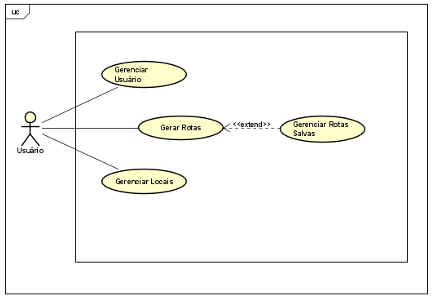
\includegraphics[width=0.8\linewidth]{imagens/caso-de-uso.png}
    \vspace{2pt}
    \footnotesize Fonte: o próprio autor (2026)
\end{figure}

\section{Especificação do caso de uso UC01: Gerenciar Locais}

O caso de uso UC01 tem como ator o Usuário e consiste na possibilidade de criar, ler, atualizar e excluir os locais que serão utilizados posteriormente na criação de rotas \cite{sriEspecUC2026}. As pré-condições estabelecem que o aplicativo deve estar aberto e que é necessária conexão à internet, uma vez que a conversão do endereço informado em coordenadas geográficas depende de serviço externo. As pós-condições preveem que um identificador de local seja gerado e que o local seja adicionado à lista exibida na tela inicial.

\subsection{Fluxo básico}

O fluxo básico descreve a sequência de eventos que deve ocorrer de forma correta para o cadastro de um novo local \cite{sriEspecUC2026}:

\begin{enumerate}
    \item o Usuário clica no botão de adição para cadastrar um novo local;
    \item o Sistema solicita as informações do local, nome e endereço;
    \item o Usuário insere as informações solicitadas e aciona a opção de salvar e buscar no mapa;
    \item o Sistema identifica se o local já existe;
    \item o Sistema adiciona o local à lista;
    \item o Usuário pode selecionar a opção de atualizar as informações do local;
    \item o Sistema valida se os campos não estão vazios e exibe um indicador de carregamento;
    \item o Sistema envia o endereço digitado para o serviço de geocodificação do OpenStreetMap (Nominatim);
    \item o Sistema recebe a latitude e a longitude correspondentes ao endereço;
    \item o Sistema salva todas as informações, nome, endereço, latitude e longitude, no banco de dados local SQLite;
    \item o Sistema fecha a tela de formulário, retorna à tela inicial e atualiza a lista, exibindo o novo ponto salvo.
\end{enumerate}

\subsection{Fluxos alternativos}

O fluxo alternativo FA01 trata da edição de um ponto existente. Na tela inicial, o Usuário aciona o ícone de edição ao lado de um ponto já salvo; o Sistema abre a tela de formulário com os dados preenchidos; o fluxo retorna ao passo 3 do fluxo básico, com a diferença de que, no passo 10, o Sistema atualiza o registro existente no banco de dados em vez de criar um novo \cite{sriEspecUC2026}.

O fluxo alternativo FA02 trata da exclusão de um ponto. Na tela inicial, o Usuário aciona o ícone de exclusão ao lado de um ponto; o Sistema remove o registro do banco de dados SQLite; e o Sistema atualiza a lista e exibe uma mensagem temporária de confirmação da exclusão \cite{sriEspecUC2026}.

O fluxo alternativo FA03 trata da visualização no mapa. Na tela inicial, o Usuário aciona o nome de um ponto salvo na lista; o Sistema abre a tela de mapa; e o Sistema renderiza o mapa centralizado na latitude e na longitude salvas, exibindo um marcador no ponto correspondente \cite{sriEspecUC2026}.

A interação entre os componentes do sistema durante o cadastro de um local é representada pelo diagrama de sequência da Figura \ref{fig:sequencia-gerenciar-locais}, que evidencia a ordem das mensagens trocadas entre a interface, a camada de persistência e o serviço de geocodificação. O ciclo de vida do local cadastrado, desde a abertura do formulário até a exclusão do registro, é representado pelo diagrama de estados da Figura \ref{fig:estado-gerenciar-locais}.

\begin{figure}[p]
    \centering
    \caption{Diagrama de sequência do caso de uso UC01}
    \label{fig:sequencia-gerenciar-locais}
    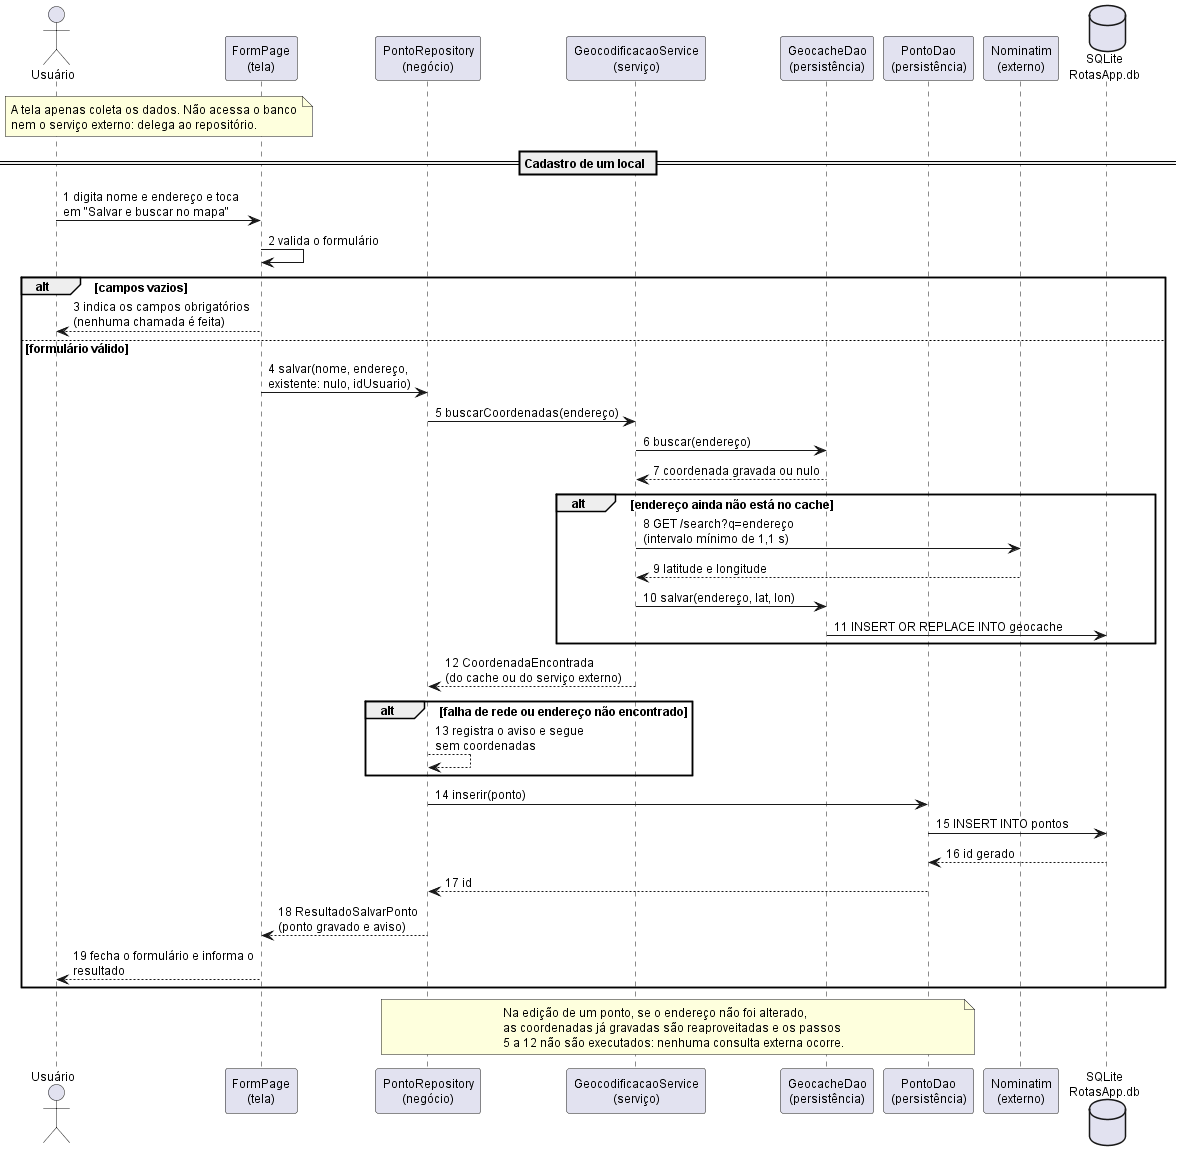
\includegraphics[angle=90,width=21cm]{imagens/sequencia-gerenciar-locais.png}
    \vspace{2pt}
    \footnotesize Fonte: o próprio autor (2026)
\end{figure}

\begin{figure}[!ht]
    \centering
    \caption{Diagrama de estados do caso de uso UC01}
    \label{fig:estado-gerenciar-locais}
    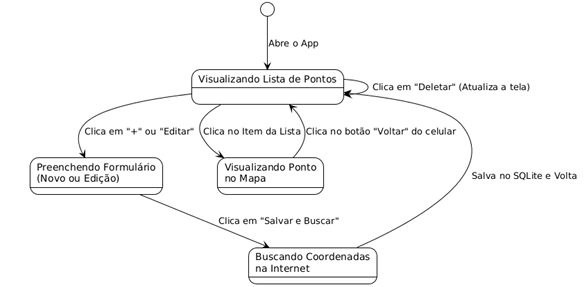
\includegraphics[width=0.8\linewidth]{imagens/estado-gerenciar-locais.png}
    \vspace{2pt}
    \footnotesize Fonte: o próprio autor (2026)
\end{figure}

\section{Demais casos de uso}

O caso de uso UC02, Gerar Rotas, tem como ator o Usuário e como pré-condição a existência de ao menos dois locais cadastrados. O fluxo principal compreende a seleção dos locais que comporão o trajeto, a escolha entre a modalidade ponto a ponto e a modalidade em circuito, o cálculo do percurso e a apresentação do resultado sobre o mapa, com a indicação da distância total e do tempo estimado de deslocamento \cite{sriEspecUC2026}.

O caso de uso UC03, Gerenciar Rotas Salvas, permite registrar um trajeto calculado para reutilização posterior e realizar as operações de consulta, atualização e exclusão sobre os registros existentes. A principal finalidade do caso de uso é eliminar a necessidade de redefinir manualmente, a cada jornada, os trajetos que se repetem com frequência na rotina do entregador \cite{sriEspecUC2026}.

O caso de uso UC04, Gerenciar Usuário, responde pelo cadastro da conta, pela autenticação e pela manutenção dos dados do usuário. O requisito de autenticação é obrigatório, de modo que não existe a possibilidade de acesso às funcionalidades do sistema sem um usuário previamente identificado \cite{sriEspecComp2025}.

\section{Modelo de classes}

O modelo de classes do sistema, apresentado na Figura \ref{fig:diagrama-de-classes}, descreve as entidades que sustentam as funcionalidades previstas e os relacionamentos existentes entre elas. A classe que representa o local cadastrado concentra os atributos de nome, endereço, latitude e longitude e mantém associação com a classe que representa a rota, uma vez que uma rota é composta por um conjunto ordenado de locais. A modelagem contempla ainda as classes responsáveis pela autenticação do usuário e pelo armazenamento das rotas salvas, cujos relacionamentos garantem que cada trajeto registrado permaneça vinculado ao usuário que o criou.

\begin{figure}[!ht]
    \centering
    \caption{Diagrama de classes do S.R.I.}
    \label{fig:diagrama-de-classes}
    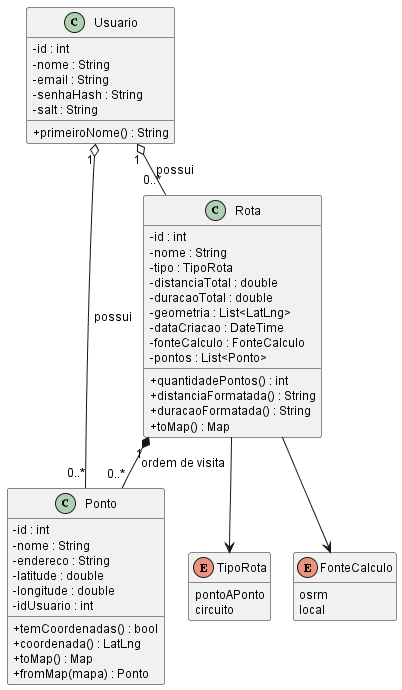
\includegraphics[width=0.56\linewidth]{imagens/diagrama-de-classes.png}
    \vspace{2pt}
    \footnotesize Fonte: o próprio autor (2026)
\end{figure}

\section{Modelo de dados}

O diagrama de entidade e relacionamento, apresentado na Figura \ref{fig:der}, representa a estrutura do banco de dados local do aplicativo. O modelo materializa as decisões do modelo de classes em tabelas, chaves primárias e relacionamentos, de modo a assegurar a integridade dos dados gravados no dispositivo.

A entidade que armazena os locais reúne o identificador do registro, o nome atribuído pelo usuário, o endereço informado e as coordenadas de latitude e longitude obtidas na geocodificação. As entidades que representam as rotas e os itens de rota permitem registrar a sequência ordenada de locais que compõe cada trajeto, preservando a ordem definida no cálculo. A entidade de usuário mantém os dados de identificação e de autenticação, e a associação entre usuário, locais e rotas garante que cada informação permaneça vinculada ao seu proprietário.

\begin{figure}[!ht]
    \centering
    \caption{Diagrama de entidade e relacionamento do S.R.I.}
    \label{fig:der}
    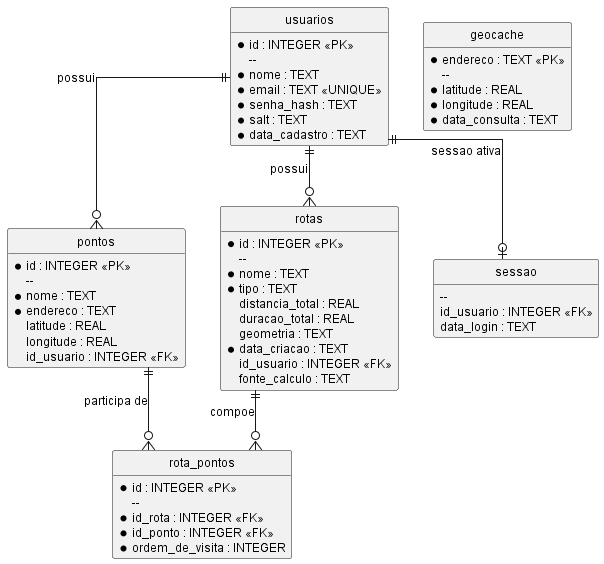
\includegraphics[width=0.8\linewidth]{imagens/der.png}
    \vspace{2pt}
    \footnotesize Fonte: o próprio autor (2026)
\end{figure}

\section{Arquitetura de implantação}

O diagrama de implantação, apresentado na Figura \ref{fig:implantacao}, descreve a distribuição dos componentes do sistema. O aplicativo é instalado no dispositivo móvel do usuário e executa de forma autônoma as funcionalidades de interface, de controle e de persistência local, apoiando-se no banco de dados SQLite embarcado. As dependências externas restringem-se aos serviços acessados pela rede: o serviço de busca e geocodificação do OpenStreetMap, responsável por converter endereços em coordenadas, o servidor de blocos cartográficos, que fornece as imagens do mapa, e o serviço de roteamento por vias, que devolve a geometria e as distâncias do trajeto calculado.

Essa distribuição de responsabilidades explica por que o cadastro de locais e a consulta aos registros permanecem funcionais mesmo em situação de conectividade intermitente, enquanto as operações de geocodificação e de cálculo de rota dependem obrigatoriamente do acesso à rede, conforme estabelecido nas premissas do produto \cite{sriVisao2025}.

\begin{figure}[!ht]
    \centering
    \caption{Diagrama de implantação do S.R.I.}
    \label{fig:implantacao}
    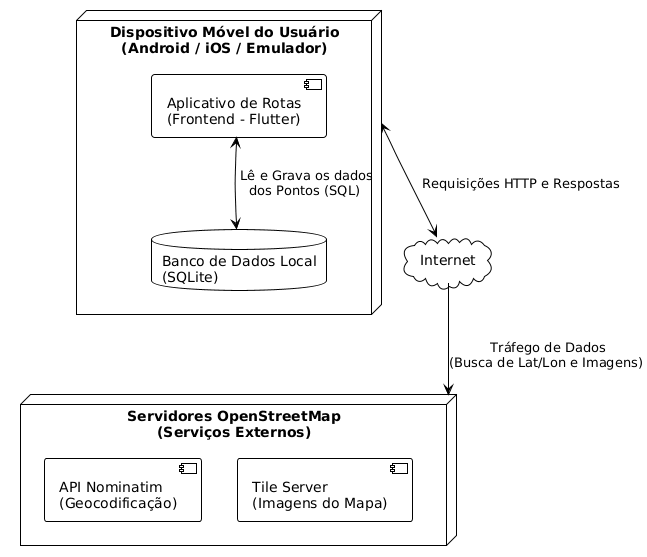
\includegraphics[width=0.8\linewidth]{imagens/implantacao.png}
    \vspace{2pt}
    \footnotesize Fonte: o próprio autor (2026)
\end{figure}

\section{Requisitos funcionais}

Os requisitos funcionais do sistema foram consolidados a partir das especificações de caso de uso e do documento de visão \cite{sriEspecUC2026, sriVisao2025}. A Tabela \ref{tab:requisitos-funcionais} apresenta os requisitos identificados e a prioridade atribuída a cada um.

\begin{table}[!ht]
    \centering
    \caption{Requisitos funcionais do S.R.I.}
    \label{tab:requisitos-funcionais}
    \begin{tabular}{p{1.4cm} p{8.6cm} p{3.4cm}}
        \hline
        \textbf{Código} & \textbf{Descrição} & \textbf{Prioridade} \\
        \hline
        RF01 & Permitir o cadastro de locais com nome, endereço e coordenadas geográficas obtidas por geocodificação. & Alta \\
        \hline
        RF02 & Permitir a consulta, a atualização e a exclusão dos locais cadastrados. & Alta \\
        \hline
        RF03 & Exibir os locais cadastrados em lista e representar cada um deles por marcador sobre o mapa. & Alta \\
        \hline
        RF04 & Gerar rotas ponto a ponto a partir da seleção de origem e destino. & Alta \\
        \hline
        RF05 & Gerar rotas em circuito, com passagem por múltiplos pontos e retorno ao ponto inicial. & Alta \\
        \hline
        RF06 & Permitir salvar as rotas geradas, bem como consultá-las, atualizá-las e excluí-las. & Média \\
        \hline
        RF07 & Permitir o cadastro e a autenticação do usuário, condicionando o acesso ao sistema à identificação prévia. & Alta \\
        \hline
        RF08 & Apresentar a distância total e o tempo estimado de deslocamento de cada rota calculada. & Média \\
        \hline
    \end{tabular}
    \vspace{2pt}
    \footnotesize Fonte: o próprio autor (2026), com base em \citeonline{sriEspecUC2026} e \citeonline{sriVisao2025}
\end{table}

\section{Requisitos não funcionais}

Os requisitos não funcionais foram extraídos da Especificação Complementar, que reúne os requisitos do sistema não capturados diretamente pelos casos de uso \cite{sriEspecComp2025}. A Tabela \ref{tab:requisitos-nao-funcionais} apresenta esses requisitos organizados por categoria.

\begin{table}[!ht]
    \centering
    \caption{Requisitos não funcionais do S.R.I.}
    \label{tab:requisitos-nao-funcionais}
    \begin{tabular}{p{3.0cm} p{10.4cm}}
        \hline
        \textbf{Categoria} & \textbf{Descrição} \\
        \hline
        Disponibilidade & O aplicativo deve estar disponível em tempo integral na sua versão mais recente, por executar de forma ativa no dispositivo móvel. \\
        \hline
        Autenticação & O acesso às funcionalidades exige usuário previamente cadastrado, não havendo possibilidade de utilização anônima. \\
        \hline
        Desempenho & O tempo para disponibilizar a resposta de uma requisição deve ser inferior a 30 segundos; requisições acima desse limite caracterizam falha de conexão entre o sistema e a fonte de dados. \\
        \hline
        Utilidade & O aplicativo opera em plataforma móvel e requer conexão de internet para o acesso aos serviços externos. \\
        \hline
        Suportabilidade & O sistema deve executar em dispositivos móveis, com hardware compatível com aplicativos de transporte, e é distribuído por meio de pacote de instalação. \\
        \hline
        Interfaces de usuário & O usuário deve realizar autenticação para acessar as funcionalidades; a interface deve ser simples e adaptada para uso em movimento. \\
        \hline
        Interfaces de hardware & O dispositivo deve dispor de acesso à internet e de receptor de GPS compatível com a operação. \\
        \hline
        Interfaces de software & A construção utiliza o framework Flutter, a linguagem Dart, o banco de dados SQLite e serviços de geolocalização, com desenvolvimento no Visual Studio Code. \\
        \hline
        Interfaces de comunicação & A comunicação entre o aplicativo e o usuário é disponibilizada integralmente pelo dispositivo móvel. \\
        \hline
        Componentes comprados & Todo o desenvolvimento foi realizado com ferramentas de código aberto; nenhum componente foi adquirido. \\
        \hline
        Licença & O sistema não exige licenças, uma vez que todos os recursos utilizados são de uso livre. \\
        \hline
        Padrões aplicáveis & A documentação e a modelagem seguem os padrões da UML e os artefatos previstos pelo processo RUP. \\
        \hline
    \end{tabular}
    \vspace{2pt}
    \footnotesize Fonte: o próprio autor (2026), com base em \citeonline{sriEspecComp2025}
\end{table}

\section{Premissas e dependências}

O documento de Visão estabelece as premissas e as dependências que condicionam a operação do sistema \cite{sriVisao2025}. Quanto às premissas, considera-se que o usuário disporá de conexão estável com a internet e de GPS ativo no dispositivo durante a utilização do aplicativo, e que o produto será compatível com as plataformas Android e iOS.

Quanto às dependências, o sistema depende de serviços externos de mapas e de geolocalização para a conversão de endereços em coordenadas e para o cálculo dos trajetos sobre a malha viária, o que vincula o comportamento das funcionalidades de rota à disponibilidade desses serviços. Estão previstas, para versões futuras, integrações com aplicativos de entrega e com sistemas de gestão logística, bem como a inclusão de recursos de visualização do tráfego em tempo real e de compartilhamento de rotas \cite{sriVisao2025}.

\chapter{Workflow \textit{as is} na notação BPMN}\label{cap:workflow-bpmn}

Este capítulo documenta o processo de negócio vigente na operação de coleta e entrega analisada, na situação em que se encontra antes da adoção do S.R.I. A descrição é apresentada na notação BPMN e serve de referência para a identificação das atividades manuais que o sistema se propõe a substituir \cite{omg2011bpmn}.

A representação do processo atual, denominada \textit{as is}, tem por finalidade explicitar não apenas a sequência das atividades, mas também a responsabilidade de cada participante e os pontos de troca de informação entre eles. Essa explicitação é o que permite reconhecer, de forma objetiva, quais etapas agregam valor à operação e quais decorrem de limitações das ferramentas empregadas \cite{omg2011bpmn}.

\section{Descrição do processo atual}

O processo atual está organizado em duas raias, que identificam os dois participantes envolvidos na operação: o Atendente, responsável pelo registro do pedido de coleta e pela organização das informações, e o Motorista, responsável pela execução do deslocamento e pela efetivação da coleta e da entrega. O diagrama correspondente é apresentado na Figura \ref{fig:workflow-as-is}.

O processo inicia-se na raia do Atendente, com a atividade \textit{Receber Pedido de Coleta}, na qual são obtidas do solicitante as informações necessárias ao atendimento. Em seguida, o Atendente executa a atividade \textit{Marcar no Quadro}, registrando manualmente, em um quadro de anotações, os dados recebidos. Esse registro constitui, na prática, a única forma de armazenamento das informações da operação.

Concluído o registro, tem início, já na raia do Motorista, a atividade \textit{Coletar Informações do Quadro}, na qual o Motorista precisa recuperar, a partir das anotações, os endereços e as demais informações referentes às coletas que lhe foram atribuídas. Como as anotações são feitas em um quadro físico, sem estrutura de dados que associe cada pedido ao seu solicitante, essa recuperação exige a leitura e a interpretação do conjunto de registros, o que introduz dependência da presença física do Motorista junto ao quadro e abre espaço para erros de transcrição e de identificação.

A etapa seguinte é a atividade \textit{Preparar Rota}. Nela, o Motorista define manualmente a ordem em que as coletas serão realizadas e elabora o trajeto correspondente, sem apoio de qualquer ferramenta de otimização. A decisão baseia-se na experiência prévia do profissional e no conhecimento que ele possui da região, o que faz com que a qualidade do trajeto varie entre motoristas e dependa da memorização de percursos anteriores.

Definida a sequência, o Motorista executa a atividade \textit{Realizar Coleta}, deslocando-se até cada ponto anotado e efetuando a coleta dos itens. Cada deslocamento entre pontos é planejado de forma isolada, uma vez que o quadro não oferece qualquer recurso de ordenação ou de visualização geográfica das paradas. Encerradas as coletas, executa-se a atividade \textit{Entregar na Agência}, que fecha o processo com o retorno do material ao ponto de origem.

\begin{figure}[p]
    \centering
    \caption{Workflow \textit{as is} do processo de coleta e entrega}
    \label{fig:workflow-as-is}
    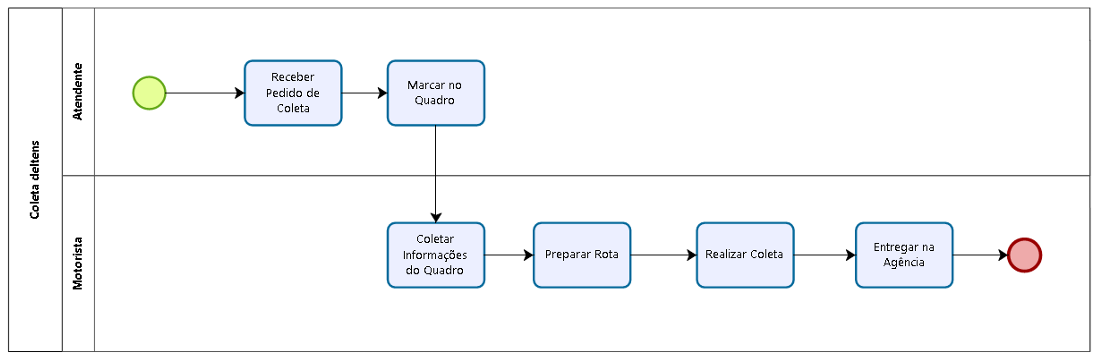
\includegraphics[angle=90,width=21cm]{imagens/workflow-as-is.png}
    \vspace{2pt}
    \footnotesize Fonte: o próprio autor (2026)
\end{figure}

\section{Ineficiências identificadas}

A análise do processo descrito permite identificar quatro ineficiências estruturais que o S.R.I. se propõe a resolver.

A primeira é a ausência de armazenamento estruturado das informações. O quadro de anotações não constitui um repositório consultável: os dados não são indexados por solicitante, não preservam histórico e não permitem busca por endereço ou por data. Essa característica obriga o registro manual repetido dos mesmos dados a cada novo pedido e impossibilita o reaproveitamento das informações em operações futuras.

A segunda é a dependência do quadro físico como intermediário. A atividade de coletar informações do quadro só pode ser executada com o Motorista presente junto às anotações, o que cria um acoplamento entre a etapa de registro e a etapa de execução que não tem correspondência com as necessidades da operação. Esse acoplamento também é a origem de erros de transcrição, uma vez que a transferência das informações ocorre por leitura humana.

A terceira é a elaboração manual da rota. Como não há ordenação automatizada das paradas, a sequência definida pelo Motorista tende a priorizar a ordem em que as coletas foram registradas ou a familiaridade com determinada região, e não a minimização da distância total percorrida. O resultado é a ocorrência de deslocamentos redundantes e de cruzamentos desnecessários de trajeto, com efeito direto sobre o consumo de combustível e sobre o tempo de operação.

A quarta é a inexistência de reutilização de trajetos. Mesmo quando a operação diária repete a mesma sequência de pontos, o processo não prevê qualquer mecanismo de armazenamento da rota definida, de modo que a atividade de preparar a rota é integralmente refeita em cada jornada. Essa repetição consome tempo de trabalho que poderia ser dedicado ao deslocamento e à entrega, além de impedir que o conhecimento acumulado pelo profissional seja preservado.

\section{Relação com a solução proposta}

Cada uma das ineficiências identificadas corresponde a um requisito do S.R.I. A ausência de armazenamento estruturado é endereçada pelo módulo de gerenciamento de locais, que substitui o quadro por registros persistidos no banco de dados local do aplicativo, indexados por identificador e pesquisáveis por nome \cite{sriEspecUC2026}. A dependência do quadro físico é eliminada pela portabilidade do dispositivo móvel, que disponibiliza as informações do local em qualquer ponto de operação, com a localização do ponto representada sobre o mapa.

A elaboração manual da rota é substituída pela funcionalidade de geração de rotas, que ordena as paradas a partir das coordenadas dos locais cadastrados e calcula o trajeto sobre a malha viária. A inexistência de reutilização de trajetos é resolvida pelo módulo de rotas salvas, que preserva o trajeto calculado e permite reexecutá-lo em outra data. Desse modo, o desenho do sistema mantém correspondência direta com o processo documentado, o que reforça a rastreabilidade entre a análise do negócio e os requisitos de software \cite{sriEspecComp2025}.

\chapter{Implementação do sistema}\label{cap:implementacao}

Este capítulo descreve a implementação do S.R.I. na versão consolidada do estágio. São apresentados a organização do código em camadas, o ambiente e as bibliotecas efetivamente utilizados, a evolução do esquema do banco de dados local, a implementação de cada caso de uso, o algoritmo de ordenação das paradas e as decisões adotadas para o tratamento de falhas. Ao final, são registrados os resultados da verificação por análise estática e por testes automatizados.

\section{Organização do código em camadas}

A versão inicial do aplicativo concentrava o acesso ao banco de dados em uma única classe e mantinha a lógica de negócio dentro das telas. À medida que os casos de uso de geração de rotas, de rotas salvas e de gerenciamento de usuário foram incorporados, essa organização passou a dificultar tanto a leitura do código quanto a sua verificação por testes. A versão consolidada adota, por isso, uma separação explícita em camadas, ilustrada na Figura \ref{fig:diagrama-de-camadas}.

\begin{figure}[!ht]
    \centering
    \caption{Organização do código em camadas}
    \label{fig:diagrama-de-camadas}
    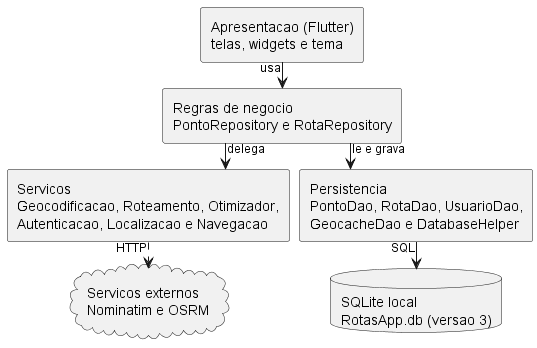
\includegraphics[width=1\linewidth]{imagens/diagrama-de-camadas.png}
    \vspace{2pt}
    \footnotesize Fonte: o próprio autor (2026)
\end{figure}

A camada de \textbf{apresentação} reúne as telas e os componentes visuais reutilizáveis. As telas não executam consultas ao banco nem chamam diretamente os serviços externos: elas solicitam operações às camadas inferiores e tratam apenas o estado da interface.

A camada de \textbf{regras de negócio} é composta pelos repositórios \texttt{PontoRepository} e \texttt{RotaRepository}. É nessa camada que residem as decisões do domínio, como reaproveitar as coordenadas já gravadas quando o endereço não foi alterado em uma edição, gravar o ponto mesmo quando a geocodificação falha e orquestrar a ordenação das paradas antes de solicitar o trajeto.

A camada de \textbf{serviços} reúne as classes com responsabilidade única e bem delimitada: a geocodificação de endereços, o cálculo de trajetos por vias, a ordenação das paradas, a autenticação, o acesso à posição do dispositivo e os cálculos da navegação assistida. Esses serviços não conhecem a interface nem gravam dados diretamente.

A camada de \textbf{persistência} contém os objetos de acesso a dados, um por conjunto de tabelas, e a classe \texttt{DatabaseHelper}, responsável exclusivamente por abrir a conexão, criar o esquema e aplicar as migrações.

A montagem das dependências é centralizada na classe \texttt{Dependencias}, que instancia os serviços e repositórios uma única vez e os entrega prontos às telas. Essa classe também é o ponto pelo qual os testes automatizados substituem o banco real por um banco em memória e o cliente HTTP real por um cliente simulado, sem que nenhuma tela precise ser alterada para isso.

\section{Ambiente e bibliotecas utilizados}

A Tabela \ref{tab:bibliotecas} relaciona as versões efetivamente utilizadas na versão consolidada, conforme registrado no arquivo de controle de dependências do projeto.

\begin{table}[!ht]
    \centering
    \caption{Bibliotecas e versões utilizadas na implementação}
    \label{tab:bibliotecas}
    \begin{tabular}{p{5cm}p{2cm}p{6cm}}
        \hline
        \textbf{Componente} & \textbf{Versão} & \textbf{Finalidade no projeto} \\
        \hline
        Flutter & 3.41.5 & Framework de interface e compilação para múltiplas plataformas \cite{flutter2024} \\
        Dart & 3.11.3 & Linguagem de programação do aplicativo \cite{dart2024} \\
        sqflite & 2.4.2 & Acesso ao banco de dados SQLite embarcado \cite{sqflite2024} \\
        flutter\_map & 8.2.2 & Renderização do mapa a partir de blocos cartográficos \cite{fluttermap2024} \\
        latlong2 & 0.9.1 & Representação de coordenadas geográficas \\
        http & 1.6.0 & Requisições aos serviços de geocodificação e de roteamento \\
        geolocator & 14.1.1 & Leitura da posição do dispositivo \cite{geolocator2024} \\
        crypto & 3.0.7 & Resumo criptográfico para a derivação da senha \\
        path & 1.9.1 & Composição do caminho do arquivo do banco de dados \\
        flutter\_lints & 5.0.0 & Regras de análise estática do código \\
        sqflite\_common\_ffi & 2.4.0+3 & Execução do SQLite nos testes automatizados \\
        \hline
    \end{tabular}
    \vspace{2pt}
    \footnotesize Fonte: o próprio autor (2026)
\end{table}

Todas as bibliotecas utilizadas são de código aberto e dispensam a contratação de licenças ou de chaves de acesso comerciais, o que atende à restrição de custo registrada na Especificação Complementar \cite{sriEspecComp2025, redhatOpenSource2024}.

\section{Evolução do esquema do banco de dados local}

O banco de dados local evoluiu em quatro versões, sempre de forma incremental e sem perda dos dados já cadastrados. A primeira versão continha apenas a tabela de pontos, correspondente ao caso de uso de gerenciamento de locais. A segunda versão acrescentou as tabelas de rotas e de itens de rota, necessárias para registrar a sequência ordenada de visitas. A terceira versão acrescentou as tabelas de usuários, de sessão e de cache de endereços, além da coluna que vincula cada ponto ao seu proprietário. A quarta versão acrescentou a tabela de preferências, que guarda a opção de manter a sessão entre execuções e a conta lembrada na tela de acesso.

A migração entre versões é aplicada pela própria classe \texttt{DatabaseHelper}, por meio do mecanismo de versionamento do SQLite. A passagem para a versão 3 utiliza a instrução de acréscimo de coluna, que preserva os registros existentes em vez de recriar a tabela. Os pontos cadastrados antes da existência de contas permanecem sem proprietário e são vinculados à primeira conta criada no dispositivo, em vez de ficarem órfãos ou inacessíveis. A passagem para a versão 4 apenas cria uma tabela nova, sem tocar nos dados existentes, de modo que a atualização é segura mesmo em um aparelho já em uso.

Duas decisões de integridade merecem registro. A primeira é a ativação explícita das chaves estrangeiras na abertura da conexão, sem a qual o SQLite aceitaria as declarações de integridade sem aplicá-las. A segunda é a gravação das rotas dentro de uma transação: como uma rota envolve a inserção em duas tabelas, a gravação atômica impede que uma falha intermediária deixe uma rota cadastrada sem os seus pontos.

\section{Implementação dos casos de uso}

\subsection{UC01: gerenciamento de locais}

O cadastro de um local solicita o nome e o endereço, converte o endereço em coordenadas por meio do serviço Nominatim e grava o registro no banco local. A tela inicial lista os pontos ordenados alfabeticamente e oferece as ações de editar, excluir e visualizar no mapa, esta última centrada nas coordenadas gravadas e com a indicação do ponto.

Duas decisões de implementação melhoram o comportamento em uso real. Na edição, quando o endereço não foi alterado, as coordenadas já gravadas são reaproveitadas e nenhuma consulta externa é realizada, o que torna a correção do nome instantânea. Além disso, se a conversão do endereço falhar, o ponto é gravado mesmo assim, sem coordenadas, e a interface informa que o endereço poderá ser localizado depois. Essa escolha preserva o cadastro em situação de conectividade instável, conforme a premissa registrada na Visão do produto \cite{sriVisao2025}.

\subsection{UC02: geração de rotas}

A montagem de uma rota ocorre em duas etapas. Na primeira, o usuário seleciona os pontos que comporão o trajeto, escolhe entre a modalidade ponto a ponto e a modalidade em circuito e, opcionalmente, define o ponto de partida e o ponto de chegada. Na segunda, o sistema apresenta o resultado do cálculo: o traçado sobre o mapa, os marcadores numerados na ordem de visita, a distância total, a duração estimada e o ganho obtido na ordenação.

A modalidade em circuito determina que o trajeto retorne ao ponto de partida, o que é obtido acrescentando-se a coordenada inicial ao final da sequência enviada ao serviço de roteamento. Qualquer alteração na seleção de pontos invalida o resultado já calculado, de modo que o usuário nunca grave uma rota diferente da que está visualizando.

A interação entre os componentes durante o cálculo é apresentada na Figura \ref{fig:sequencia-gerar-rota}. O diagrama evidencia a separação de responsabilidades entre a tela, o repositório, o serviço de ordenação, o serviço de roteamento e o objeto de acesso a dados, e mostra os dois desvios previstos: a recusa do cálculo quando a seleção é insuficiente e o recuo para a estimativa local quando o serviço de roteamento não responde. A gravação aparece como um trecho opcional, que só ocorre depois que o usuário confirma a operação, e é executada dentro de uma transação.

\begin{figure}[p]
    \centering
    \caption{Diagrama de sequência do caso de uso UC02 (geração de rotas)}
    \label{fig:sequencia-gerar-rota}
    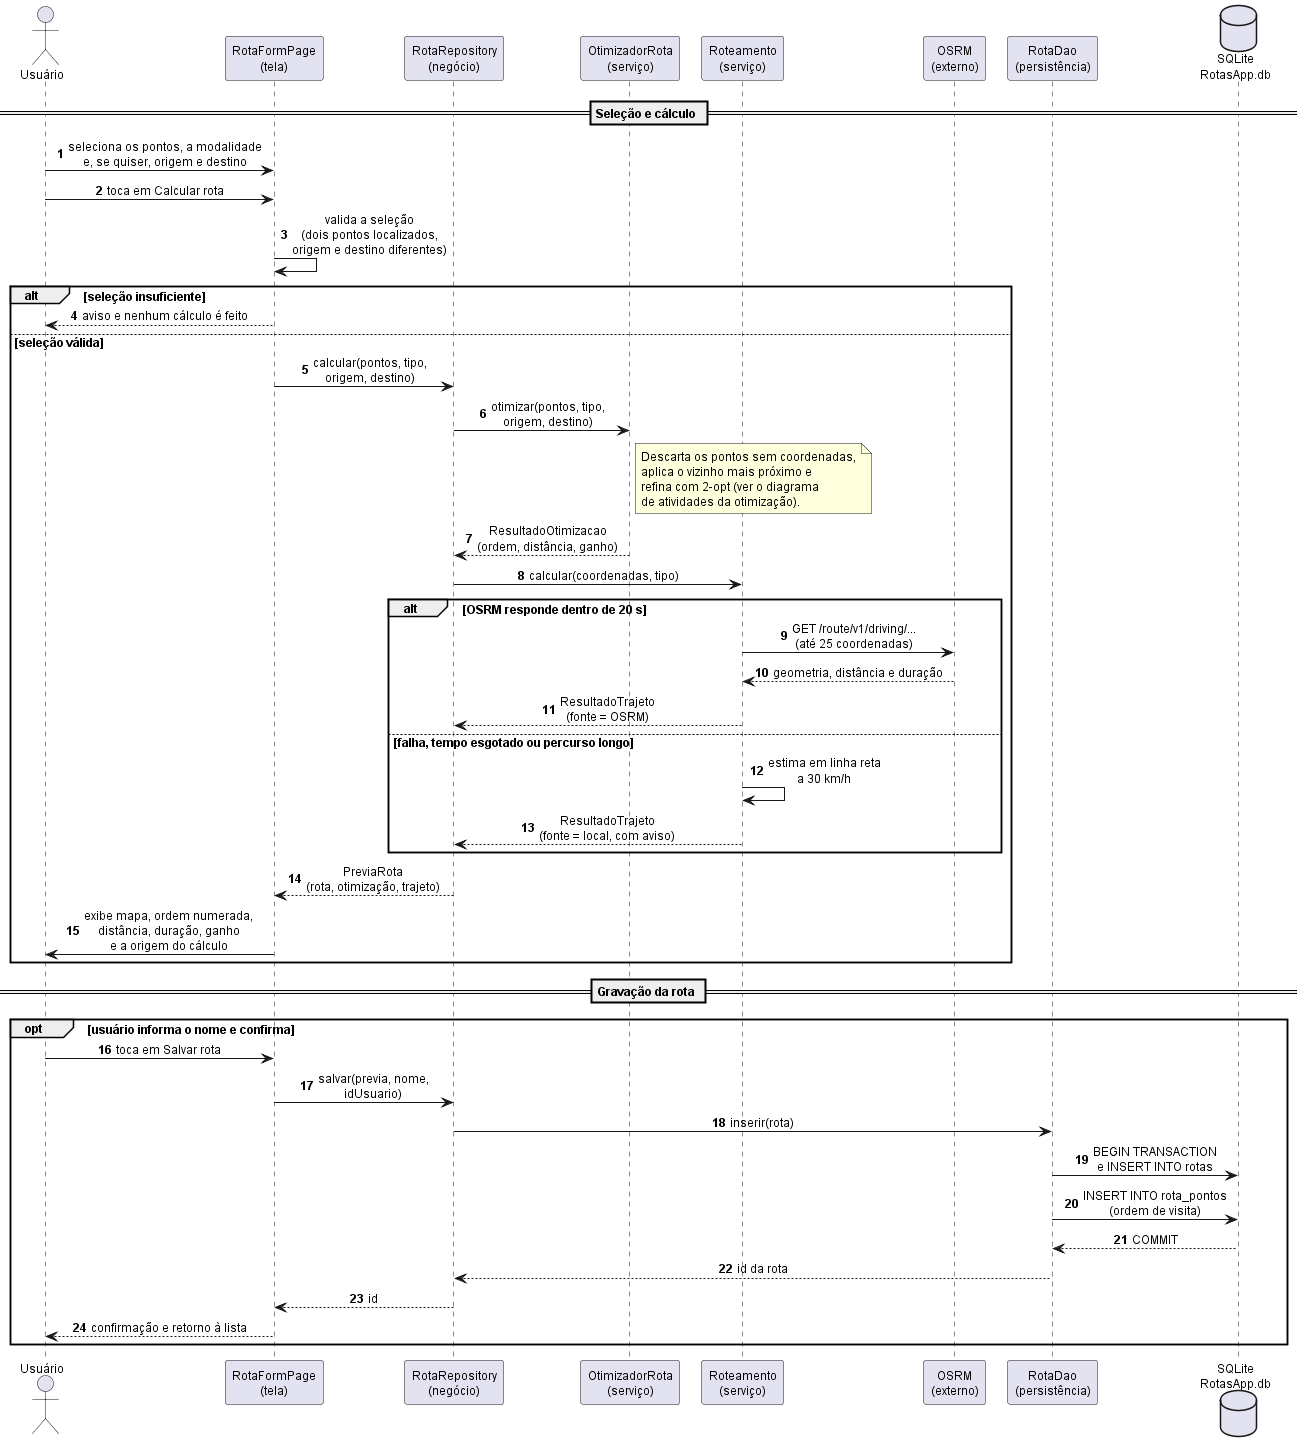
\includegraphics[width=\linewidth]{imagens/sequencia-gerar-rota.png}
    \vspace{2pt}
    \footnotesize Fonte: o próprio autor (2026)
\end{figure}

\subsection{UC03: gerenciamento de rotas salvas}

As rotas calculadas podem ser nomeadas e gravadas para reutilização. A listagem das rotas salvas apresenta o nome, a modalidade, a quantidade de paradas, a distância e a duração, e oferece as operações de consulta, de edição e de exclusão. A consulta de uma rota salva exibe novamente o traçado sobre o mapa e a ordem de visita, e é o ponto de partida para a navegação assistida.

A gravação da rota persiste a sua geometria, de modo que a reabertura de um trajeto já calculado não exige uma nova consulta ao serviço externo. A exclusão de um ponto cadastrado remove automaticamente o vínculo desse ponto com as rotas que o utilizavam, sem eliminar as rotas remanescentes.

\subsection{UC04: gerenciamento de usuário}

O acesso ao aplicativo exige autenticação prévia, conforme estabelecido na Especificação Complementar \cite{sriEspecComp2025}. A implementação compreende a criação de conta, o acesso, a manutenção dos dados cadastrais, a troca de senha e a exclusão da conta.

A senha não é armazenada em texto legível. Para cada conta é sorteado um sal aleatório de dezesseis bytes, e o valor gravado resulta da aplicação repetida do resumo criptográfico SHA-256, em dez mil iterações, sobre a composição do sal com a senha. Essa repetição, denominada alongamento de chave, encarece substancialmente a tentativa de adivinhação por força bruta. Trata-se de um esquema didático: um sistema em produção deveria empregar algoritmos projetados especificamente para senhas, como PBKDF2, bcrypt ou Argon2. A comparação entre o valor calculado e o valor gravado é feita sem interrupção na primeira diferença, de modo que o tempo de resposta não revele quantos caracteres iniciais estavam corretos.

A sessão do usuário é registrada em uma tabela de linha única, o que permite restaurar o acesso quando o aplicativo é reaberto sem manter a senha em memória. A mensagem devolvida em uma tentativa de acesso malsucedida é idêntica para e-mail inexistente e para senha incorreta, o que evita revelar quais endereços estão cadastrados no aparelho.

Como a autenticação é obrigatória, a tela de acesso foi construída para exigir o mínimo de digitação, de modo que a exigência não se transforme em atrito diário. Duas medidas atendem a esse objetivo.

A primeira é a \textbf{conta lembrada}: o e-mail e o nome do último acesso são gravados na tabela de preferências, e a tela de acesso passa a exibir um cartão de identificação da conta no lugar do campo de e-mail. O usuário digita apenas a senha, e o foco já começa nesse campo, de modo que o acesso se completa com o próprio botão de confirmação do teclado. Um botão de troca de conta permite informar outro usuário quando necessário.

A segunda é a opção \textbf{manter conectado}, marcada por padrão. Quando está marcada, a sessão é gravada no banco e o aplicativo abre direto no conteúdo nas execuções seguintes; quando não está, nenhuma sessão é gravada e a senha volta a ser pedida na próxima abertura, ainda com o e-mail lembrado. Para que esse comportamento funcione sem depender do banco, o usuário autenticado é mantido em memória na tela que decide entre o acesso e o conteúdo, e a gravação da sessão é tratada como uma decisão à parte.

Um efeito colateral desse desenho merece registro: como a sessão pode não estar gravada, a tela que decide o que exibir não pode simplesmente reler o banco após o acesso — ela precisa receber o usuário autenticado como resultado da operação. Essa foi a mudança estrutural necessária para suportar a opção.

A Figura \ref{fig:sequencia-autenticacao} detalha esse fluxo. O diagrama cobre a abertura da tela com a leitura da conta lembrada, a tentativa de acesso com as duas ramificações de falha e de sucesso, a comparação da senha derivada em tempo constante e a decisão entre gravar ou não a sessão, além da atualização da conta lembrada nas preferências. A nota inicial registra que a decisão entre apresentar o acesso ou o conteúdo pertence ao portão de sessão, e não à tela de acesso.

\begin{figure}[p]
    \centering
    \caption{Diagrama de sequência do caso de uso UC04 (autenticação)}
    \label{fig:sequencia-autenticacao}
    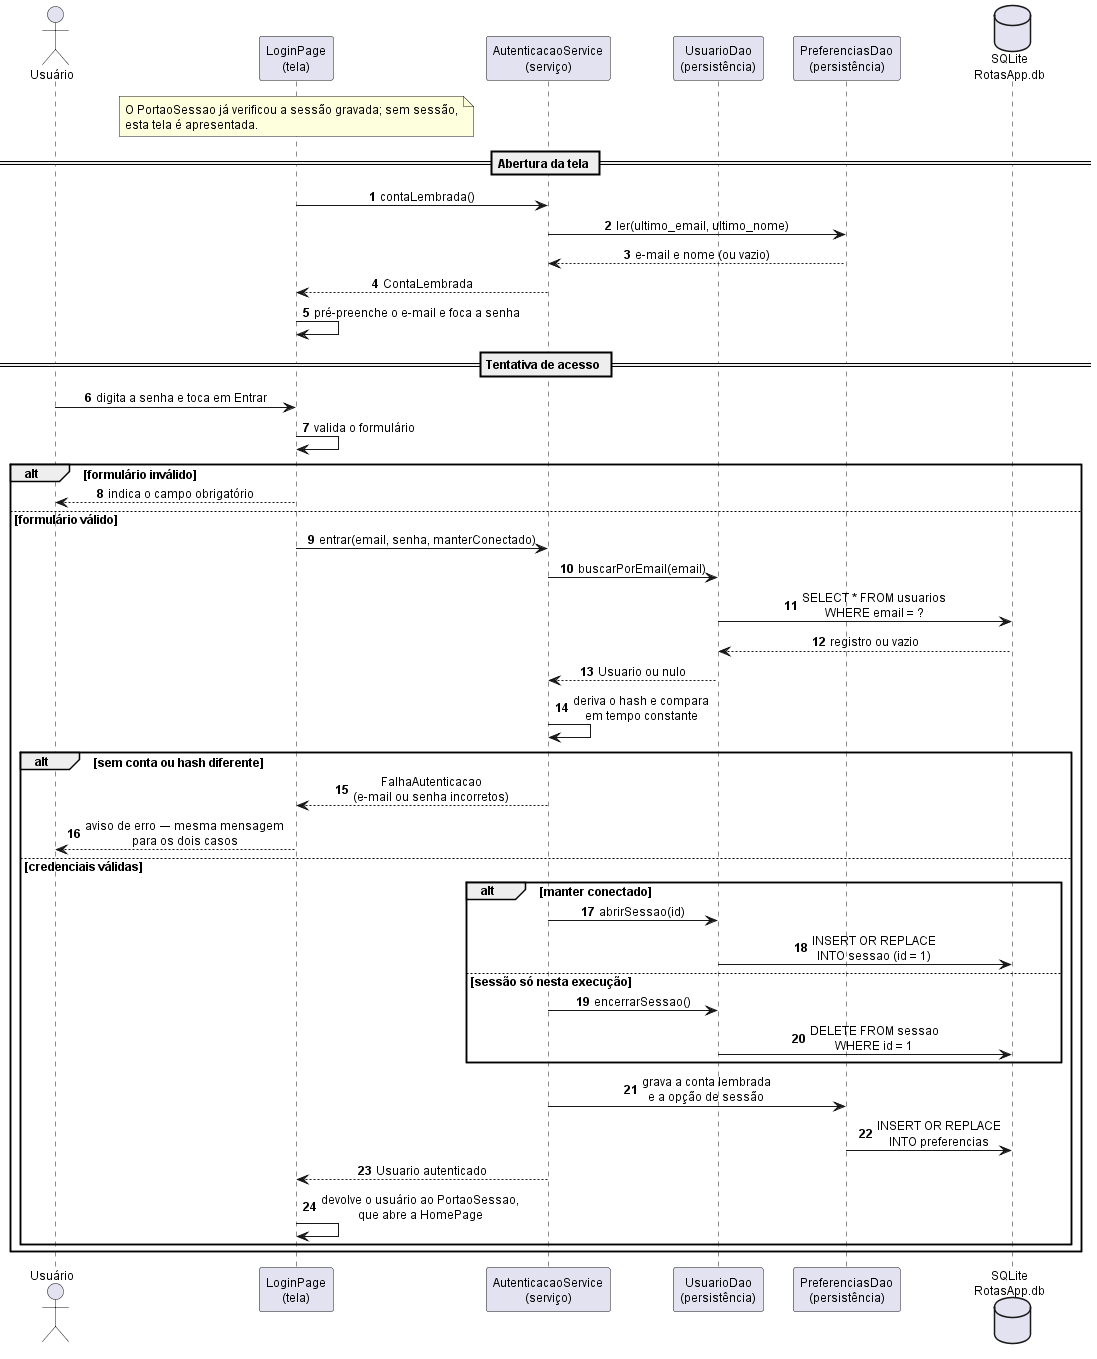
\includegraphics[width=1\linewidth]{imagens/sequencia-autenticacao.png}
    \vspace{2pt}
    \footnotesize Fonte: o próprio autor (2026)
\end{figure}

\subsection{Navegação assistida}

A navegação assistida acompanha a posição do veículo durante a execução da rota. A tela mantém em destaque o próximo ponto da ordem de visita, informa a distância e o sentido até ele e apresenta o trajeto completo sobre o mapa, com a posição atual do veículo em sobreposição às paradas.

O avanço entre paradas é automático: quando o veículo entra em um raio de cinquenta metros do ponto-alvo, o sistema passa a apontar para a parada seguinte e comunica a chegada. Esse raio foi adotado por ser compatível com a precisão do sinal de GPS em área urbana e com a extensão de um quarteirão, evitando exigir que o motorista pare exatamente sobre a coordenada. Como a precisão do sinal pode ser insuficiente em determinados trechos, a tela também permite avançar manualmente para a próxima parada.

Registra-se, com clareza, que se trata de uma navegação assistida e não de uma navegação curva a curva: o sistema não recalcula o trajeto a cada desvio da malha viária nem emite comandos de voz. O que a funcionalidade resolve é o problema identificado no levantamento de requisitos, que é manter o motorista informado sobre qual é a próxima entrega e quanto falta para alcançá-la, aproveitando a ordem de visita já otimizada e o traçado previamente gravado.

\section{Ordenação das paradas}

A ordem de visita dos pontos é definida pelo \texttt{OtimizadorRotaService}. Determinar a menor rota que visita um conjunto de pontos e retorna ao início corresponde ao problema do caixeiro-viajante, cuja solução exata é inviável para instâncias de tamanho realista, pois o número de ordens possíveis cresce de forma fatorial. A estratégia adotada é, portanto, heurística e opera em duas etapas.

A primeira etapa é construtiva e emprega a heurística do vizinho mais próximo: partindo do ponto de origem, escolhe-se sempre o ponto ainda não visitado mais próximo do atual. O procedimento tem custo quadrático no número de pontos e produz rapidamente uma solução válida, mas tende a deixar um trecho longo para o final, pois as escolhas locais não consideram o fechamento do percurso.

A segunda etapa refina a solução por meio do método 2-opt: procura-se um par de arestas cuja troca encurte o percurso e, quando esse par é encontrado, o trecho entre elas é invertido. O procedimento se repete até que nenhuma inversão produza ganho. Nas rotas em circuito, o percurso é tratado como um ciclo cujo ponto de partida permanece fixo; nas rotas ponto a ponto, tanto o ponto de partida quanto o de chegada são preservados, pois representam a escolha explícita do usuário. O número de inversões aplicadas e a redução obtida são registrados e apresentados ao usuário, o que torna o efeito do refinamento verificável na própria interface.

O fluxo completo do algoritmo é apresentado na Figura \ref{fig:atividades-otimizacao}. O diagrama mostra a validação de entrada, a fixação dos pontos que não podem mudar de posição, as duas etapas de construção e refinamento com os seus laços de repetição e as condições de parada, além do resultado devolvido ao repositório. Os pontos de decisão correspondem exatamente às guardas implementadas no serviço: a exigência de ao menos dois pontos com coordenadas, o critério de ganho do 2-opt e o limite de passagens que evita laços longos.

\begin{figure}[!ht]
    \centering
    \caption{Fluxo do algoritmo de ordenação das paradas}
    \label{fig:atividades-otimizacao}
    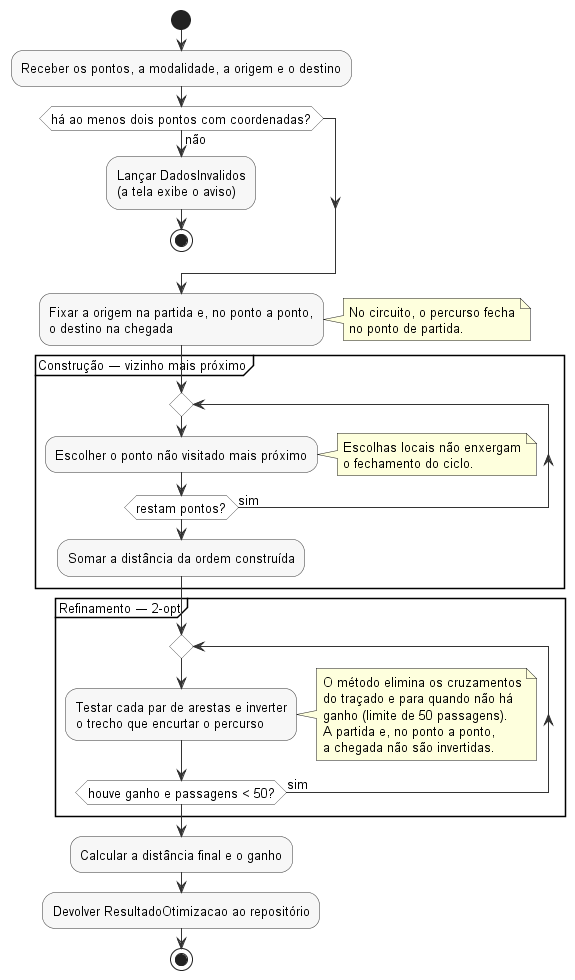
\includegraphics[width=1\linewidth]{imagens/atividades-otimizacao.png}
    \vspace{2pt}
    \footnotesize Fonte: o próprio autor (2026)
\end{figure}

A qualidade do resultado é verificada por teste automatizado que compara a distância obtida pela heurística com a menor distância possível, calculada por força bruta sobre todas as ordens de visita de uma instância pequena. O teste exige que a solução heurística não seja inferior ao ótimo, o que seria impossível, e que não exceda o ótimo em mais de quinze por cento.

\section{Tratamento de falhas e degradação controlada}

Os requisitos de confiabilidade preveem tolerância a falhas de rede e recuperação da rota \cite{sriVisao2025}. A implementação atende a esse requisito por meio de três mecanismos.

O primeiro é o recuo para o cálculo local. Quando o serviço de roteamento não responde, o trajeto é estimado em linha reta a partir das coordenadas, com a duração calculada pela velocidade urbana média assumida de trinta quilômetros por hora. A origem do cálculo é gravada junto com a rota e informada na interface, de modo que o usuário saiba que o traçado apresentado não segue as vias reais e possa recalcular o trajeto quando houver conexão.

O segundo é o limite de tempo das requisições externas. O serviço de roteamento é consultado com limite de vinte segundos, valor deliberadamente inferior aos trinta segundos estabelecidos como requisito de desempenho \cite{sriEspecComp2025}, para que mesmo o pior caso, que é o recuo para a estimativa local, permaneça dentro do prazo aceitável.

O terceiro é o controle de uso do serviço de geocodificação. A política de uso do Nominatim recomenda no máximo uma requisição por segundo por aplicação. O serviço implementado impõe um intervalo mínimo entre consultas externas e mantém um cache local dos endereços já convertidos, de modo que a repetição de um mesmo endereço não gera tráfego e o formulário responde de imediato.

As falhas são traduzidas, nos serviços, para exceções de domínio que já carregam uma mensagem em português adequada ao usuário, enquanto o detalhe técnico é preservado para depuração. Nenhuma tela exibe ao usuário o texto cru de um erro de rede ou de banco de dados.

\section{Verificação por análise estática e testes automatizados}

A verificação do código foi conduzida em dois níveis automatizados. O primeiro é a análise estática, executada pela ferramenta de análise do ambiente Flutter com as regras do conjunto \texttt{flutter\_lints}: a versão consolidada do código não apresenta nenhum aviso nem erro. Essa análise cobre erros de tipagem, uso incorreto de contexto de interface após operações assíncronas, importações não utilizadas e demais más práticas verificáveis sem execução.

O segundo nível é a suíte de testes automatizados, composta por cento e oito testes distribuídos em seis arquivos, conforme a Tabela \ref{tab:testes}. Os testes de persistência e de autenticação executam contra um banco SQLite em memória criado com o mesmo esquema e as mesmas migrações utilizados em produção, o que garante que a verificação incida sobre o esquema real e não sobre uma cópia que poderia divergir. As chamadas aos serviços externos são substituídas por respostas simuladas, de modo que os testes não dependem de rede e são determinísticos.

\begin{table}[!ht]
    \centering
    \caption{Distribuição dos testes automatizados}
    \label{tab:testes}
    \begin{tabular}{p{5cm}p{2cm}p{8cm}}
        \hline
        \textbf{Arquivo} & \textbf{Testes} & \textbf{O que verifica} \\
        \hline
        geo\_utils\_test.dart & 20 & Distâncias pela fórmula de Haversine contra valores conhecidos, formatação de distância e duração, leitura e gravação da geometria e tolerância a registros corrompidos \\
        otimizador\_rota\_test.dart & 9 & Corretude do refinamento 2-opt em ordens cruzadas, preservação dos pontos de partida e chegada, descarte de pontos sem coordenadas e proximidade do ótimo obtido por força bruta \\
        navegacao\_test.dart & 16 & Avanço entre paradas pelo raio de chegada, instrução apresentada, distância restante em rotas abertas e em circuitos e cálculo do progresso \\
        autenticacao\_test.dart & 25 & Derivação e comparação de senha, validações de cadastro, vínculo dos pontos legados, troca de senha, exclusão de conta, identidade das mensagens de erro, conta lembrada e política de sessão \\
        persistencia\_test.dart & 30 & Criação do esquema, migração da versão 1 preservando os dados, operações de cada objeto de acesso a dados, preferências, integridade referencial, transação de gravação de rota, cache e limites de uso da geocodificação e recuo do roteamento \\
        widget\_test.dart & 8 & Validação do formulário de acesso, fluxo completo de criação de conta até a tela inicial e acesso com conta lembrada, todos com banco em memória \\
        \hline
        \textbf{Total} & \textbf{108} & \\
        \hline
    \end{tabular}
    \vspace{2pt}
    \footnotesize Fonte: o próprio autor (2026)
\end{table}

Além desses dois níveis, a compilação completa do aplicativo foi executada com sucesso para dois alvos distintos: o alvo web, que confirma que o conjunto do código-fonte compila de ponta a ponta, e o alvo Android, cujo pacote de instalação foi gerado sem falhas. A geração do pacote Android constituiu a verificação mais exigente, porque envolve, além da compilação do código Dart, a compilação do código nativo, a validação do manifesto de permissões e a vinculação das bibliotecas de plataforma usadas pelo acesso ao banco de dados e à localização.

Sobre essa base, a execução funcional foi verificada em emulador Android, com o aplicativo instalado e operado nos fluxos descritos na especificação de caso de uso. A verificação cobriu a criação de conta e a abertura de sessão, o cadastro de pontos, a conversão de endereços em coordenadas pelo serviço Nominatim, a renderização do mapa com os blocos cartográficos e o marcador do ponto, a geração de uma rota em circuito com quatro paradas, a gravação e a reabertura da rota salva e a navegação assistida, incluindo a solicitação e a concessão da permissão de localização e o avanço automático entre paradas. Nessa execução o cálculo da rota foi efetivamente resolvido pelo serviço de roteamento, e não pelo recuo local: o resultado registrado foi de 23,9 quilômetros, 40 minutos de duração estimada e traçado sobre as vias reais de Londrina, o que confirma a integração com o serviço externo.

Um comportamento observado nessa execução merece registro, por validar a estratégia de migração descrita na seção anterior. Ao instalar a versão consolidada sobre um banco criado pela primeira versão do aplicativo, os pontos então existentes, que não possuíam proprietário, foram vinculados à primeira conta criada no dispositivo e passaram a aparecer na lista do usuário, em vez de ficarem órfãos ou inacessíveis. A migração, portanto, foi exercitada sobre dados reais e não apenas sobre um banco de teste.

A política de sessão também foi verificada nos dois sentidos. Com a opção de manter conectado marcada, o aplicativo foi encerrado e reaberto e apresentou diretamente a lista de pontos, sem passar pela tela de acesso. Com a opção desmarcada, o encerramento e a reabertura devolveram a tela de acesso, porém com a conta já identificada e apenas o campo de senha a preencher — ou seja, o atrito fica restrito à digitação da senha, e não à identificação da conta.

Cabe registrar o que permanece pendente. A execução em emulador não reproduz as condições de campo: a variação real da precisão do sinal de GPS, o comportamento em conectividade intermitente e o consumo de energia só podem ser avaliados em aparelho físico, em uso prolongado. Além disso, as métricas de tempo de resposta e de assertividade declaradas nos requisitos dependem de medição sistemática em campo e da validação das rotas junto ao usuário, o que está previsto como continuidade do trabalho.

\section{Interface do aplicativo}

As telas da versão consolidada são apresentadas nas Figuras \ref{fig:tela-login} a \ref{fig:tela-navegacao}. Todas as capturas foram obtidas do aplicativo em execução no emulador, com dados de demonstração cadastrados, e não de protótipos.

A Figura \ref{fig:tela-login} apresenta a tela de acesso. O aplicativo abre nessa tela sempre que não há sessão ativa, o que materializa o requisito de autenticação obrigatória: não existe caminho de acesso às funcionalidades sem a identificação do usuário. A conta do último acesso aparece identificada no topo, de modo que resta ao usuário digitar apenas a senha, e a opção de manter a sessão entre execuções vem marcada por padrão.

\begin{figure}[!ht]
    \centering
    \caption{Tela de acesso ao sistema}
    \label{fig:tela-login}
    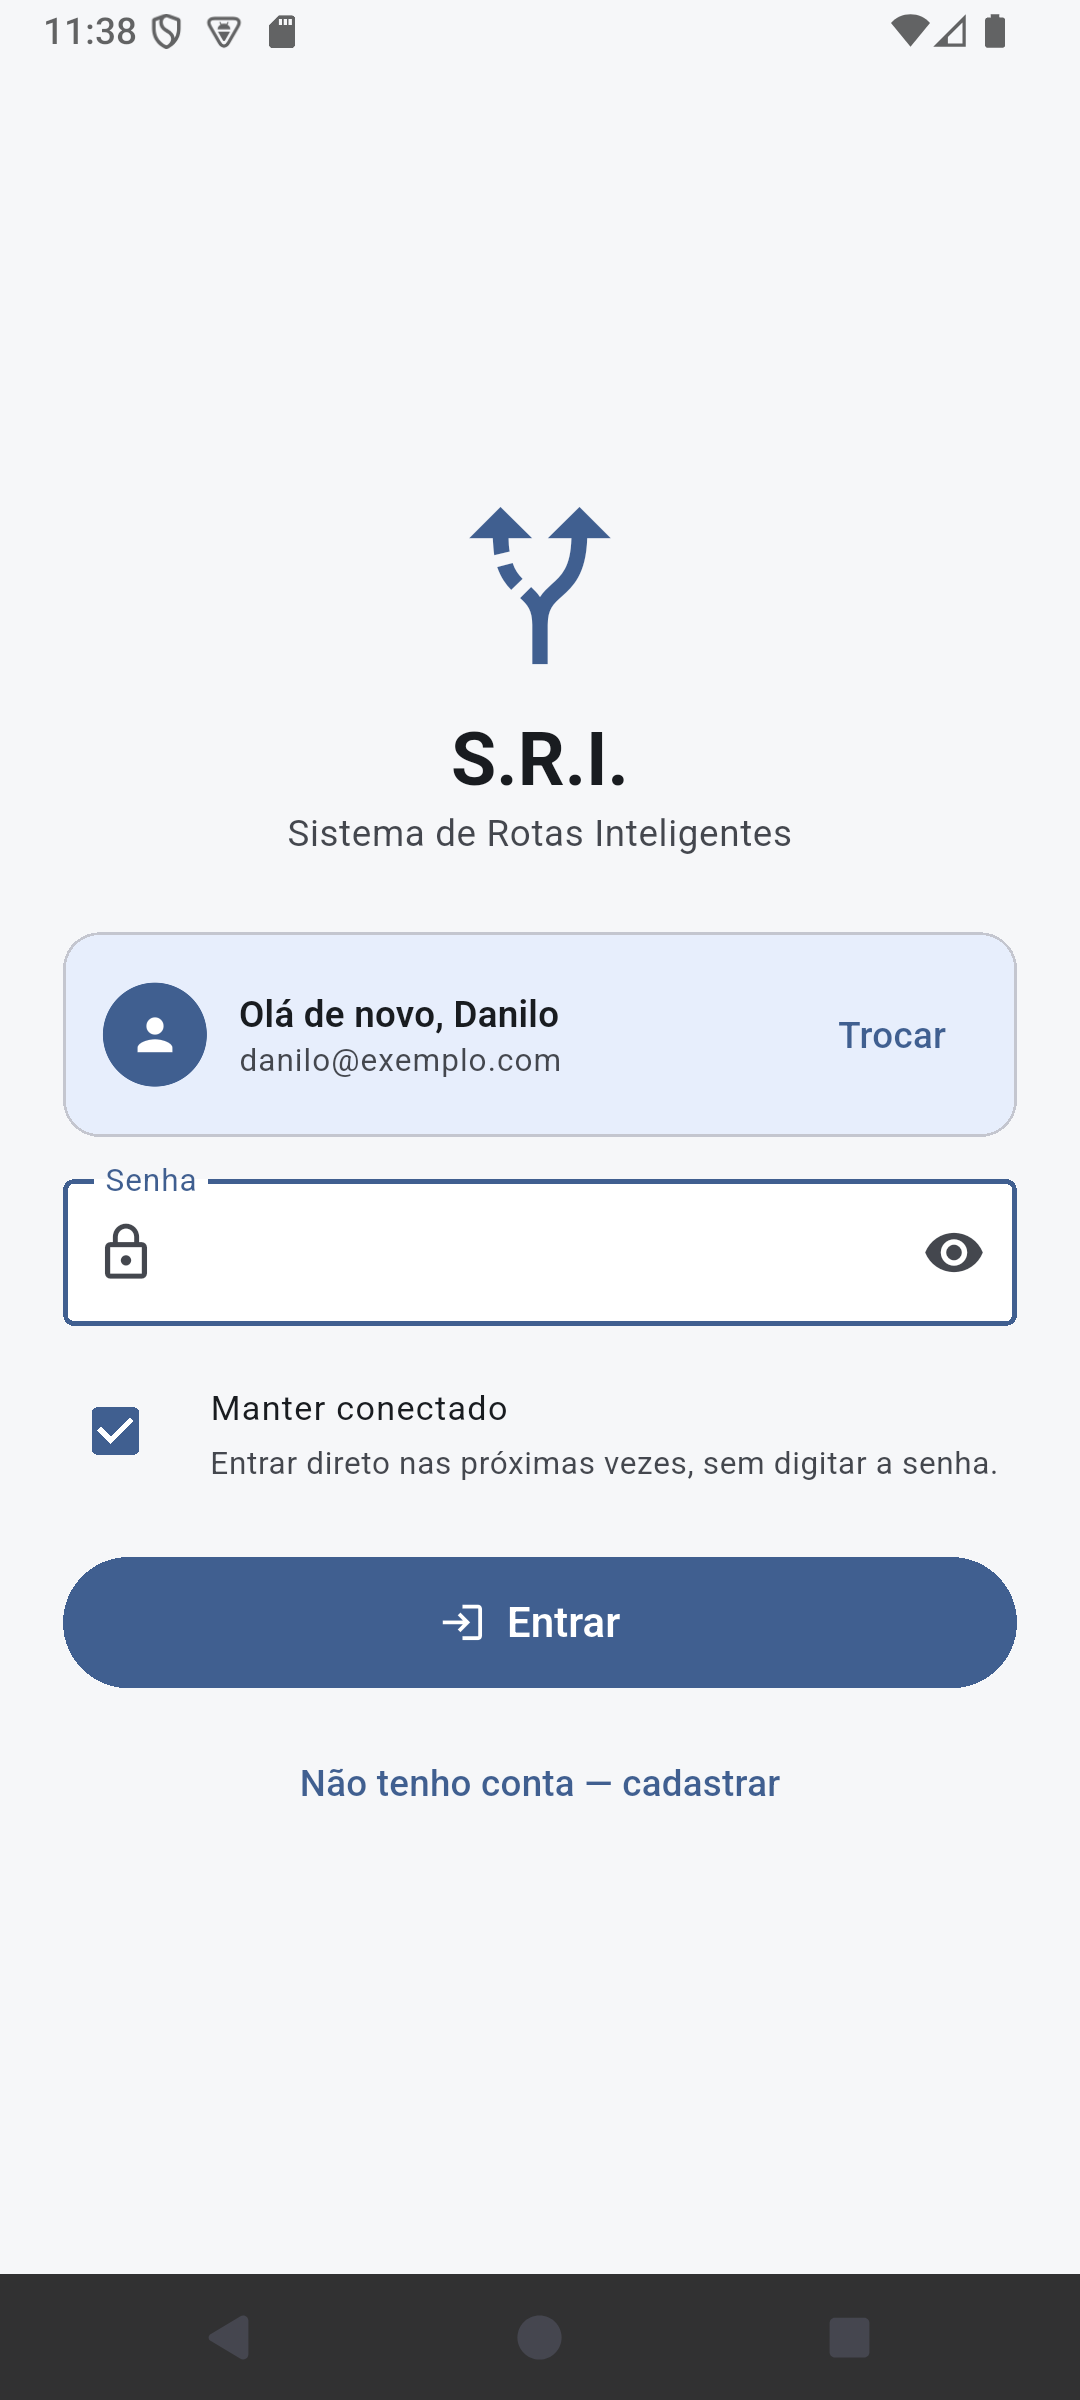
\includegraphics[width=0.5\linewidth]{imagens/tela-login.png}
    \vspace{2pt}
    \footnotesize Fonte: captura do aplicativo em execução (2026)
\end{figure}

A Figura \ref{fig:tela-pontos} apresenta a lista de pontos cadastrados, com o nome, o endereço e as ações de editar e excluir, além do indicador de que o endereço já foi localizado no mapa. O acesso ao mapa de cada ponto se dá pelo toque sobre o item da lista.

\begin{figure}[!ht]
    \centering
    \caption{Tela de pontos cadastrados}
    \label{fig:tela-pontos}
    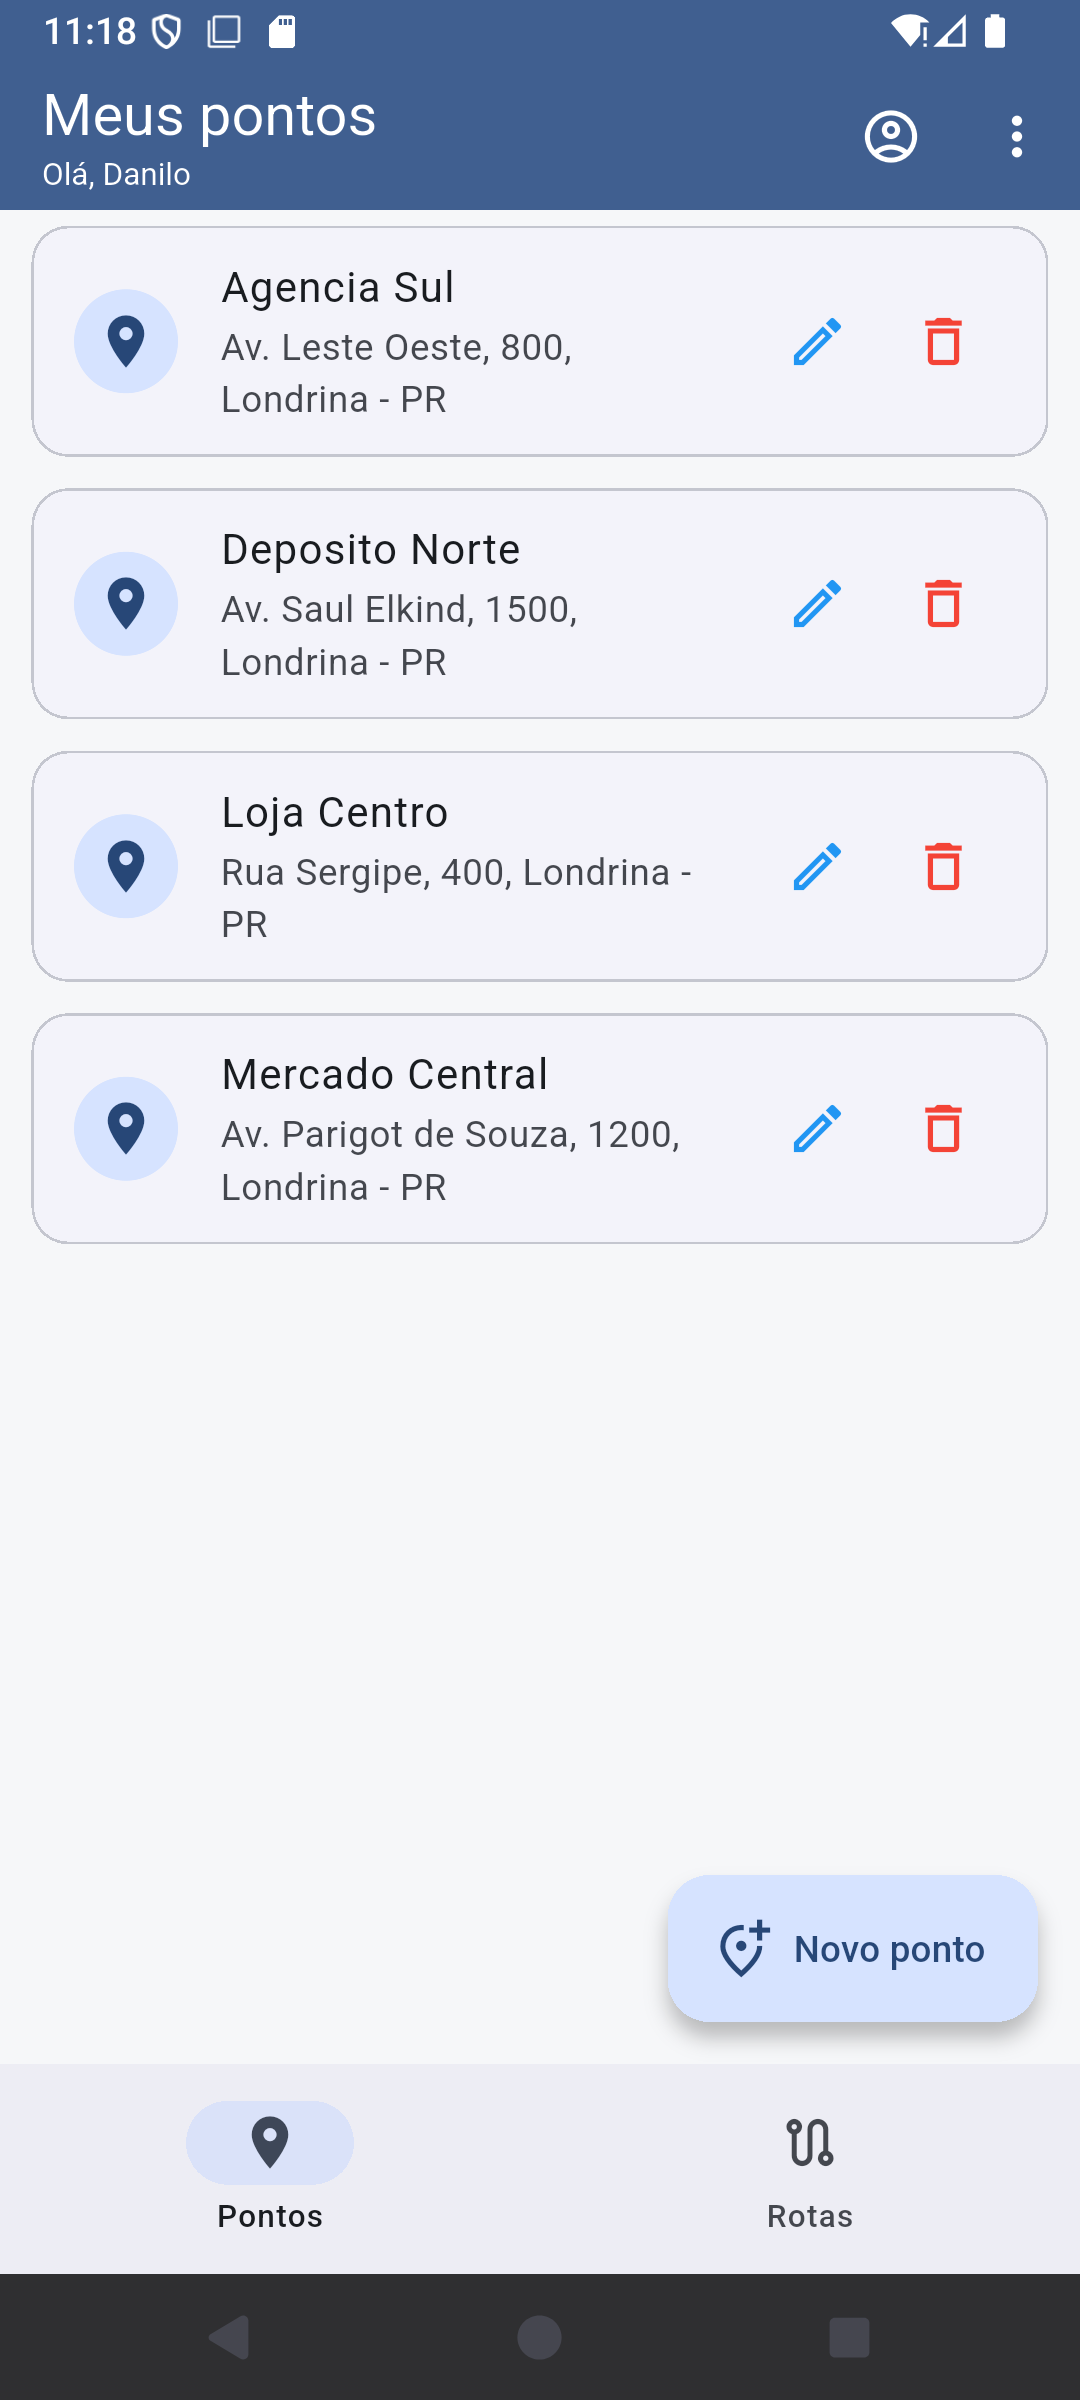
\includegraphics[width=0.5\linewidth]{imagens/tela-pontos.png}
    \vspace{2pt}
    \footnotesize Fonte: captura do aplicativo em execução (2026)
\end{figure}

A Figura \ref{fig:tela-previa-rota} apresenta o resultado do cálculo de uma rota em circuito com quatro paradas. A tela reúne o traçado sobre o mapa, as métricas do percurso, o modo de operação, a origem efetiva do cálculo e a ordem de visita otimizada, com a indicação da partida, das paradas intermediárias e do retorno que fecha o circuito.

\begin{figure}[!ht]
    \centering
    \caption{Prévia de rota em circuito calculada}
    \label{fig:tela-previa-rota}
    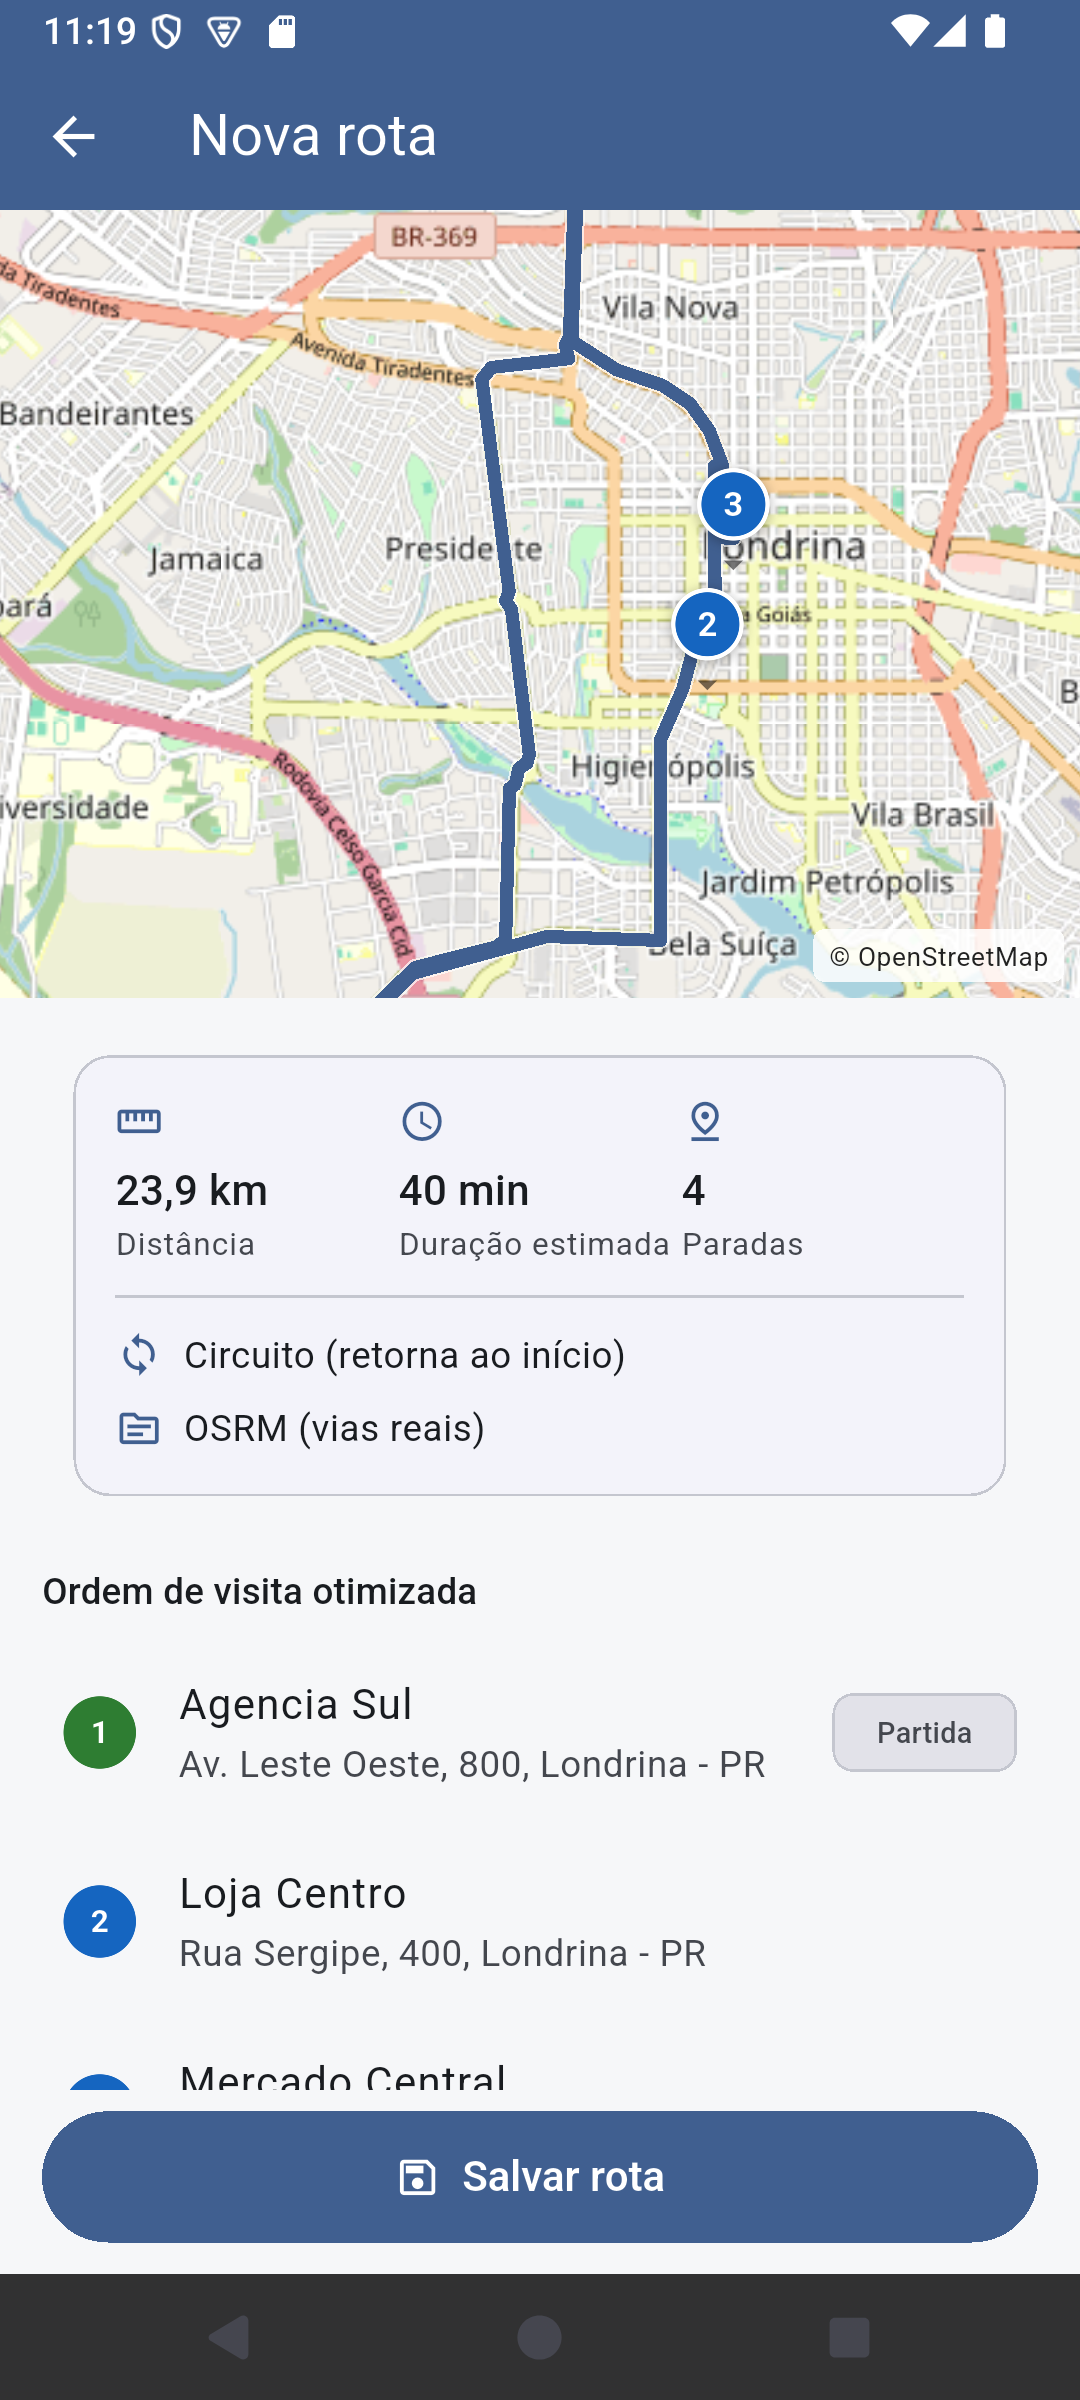
\includegraphics[width=0.5\linewidth]{imagens/tela-previa-rota.png}
    \vspace{2pt}
    \footnotesize Fonte: captura do aplicativo em execução (2026)
\end{figure}

A Figura \ref{fig:tela-rotas-salvas} apresenta a lista de rotas salvas, com a modalidade, a quantidade de paradas, a distância e a duração de cada trajeto, além das ações de edição e de exclusão.

\begin{figure}[!ht]
    \centering
    \caption{Tela de rotas salvas}
    \label{fig:tela-rotas-salvas}
    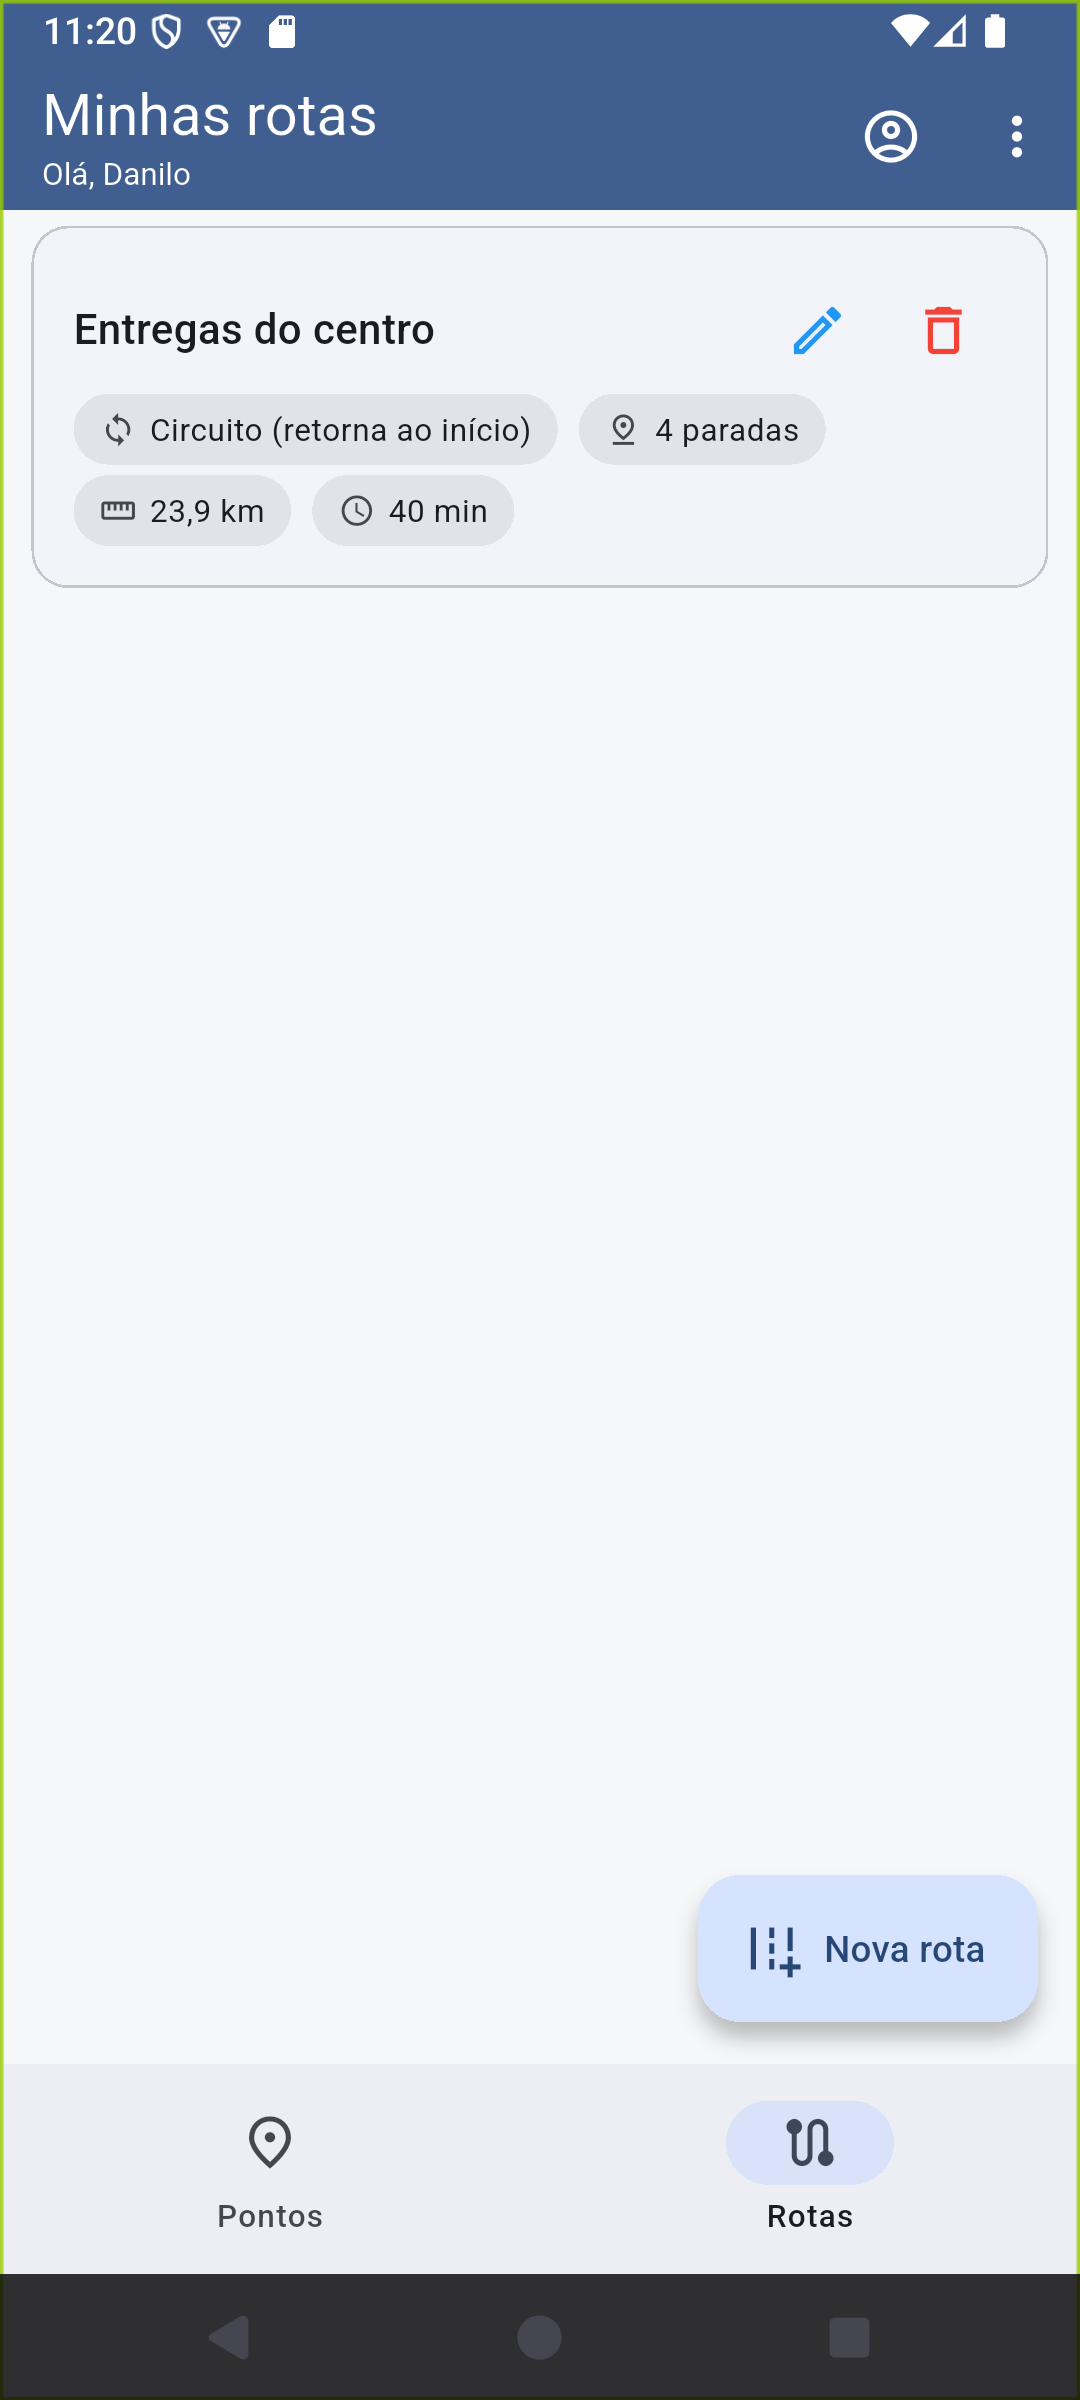
\includegraphics[width=0.5\linewidth]{imagens/tela-rotas-salvas.png}
    \vspace{2pt}
    \footnotesize Fonte: captura do aplicativo em execução (2026)
\end{figure}

A Figura \ref{fig:tela-navegacao} apresenta a navegação assistida em curso. A faixa superior traz a instrução do próximo ponto, com a distância e o sentido; o mapa exibe o traçado e a posição atual do veículo; e o painel inferior informa a parada em curso, a distância restante, o progresso do percurso e as ações de centralizar o mapa e de avançar manualmente para a próxima parada.

\begin{figure}[!ht]
    \centering
    \caption{Tela de navegação assistida}
    \label{fig:tela-navegacao}
    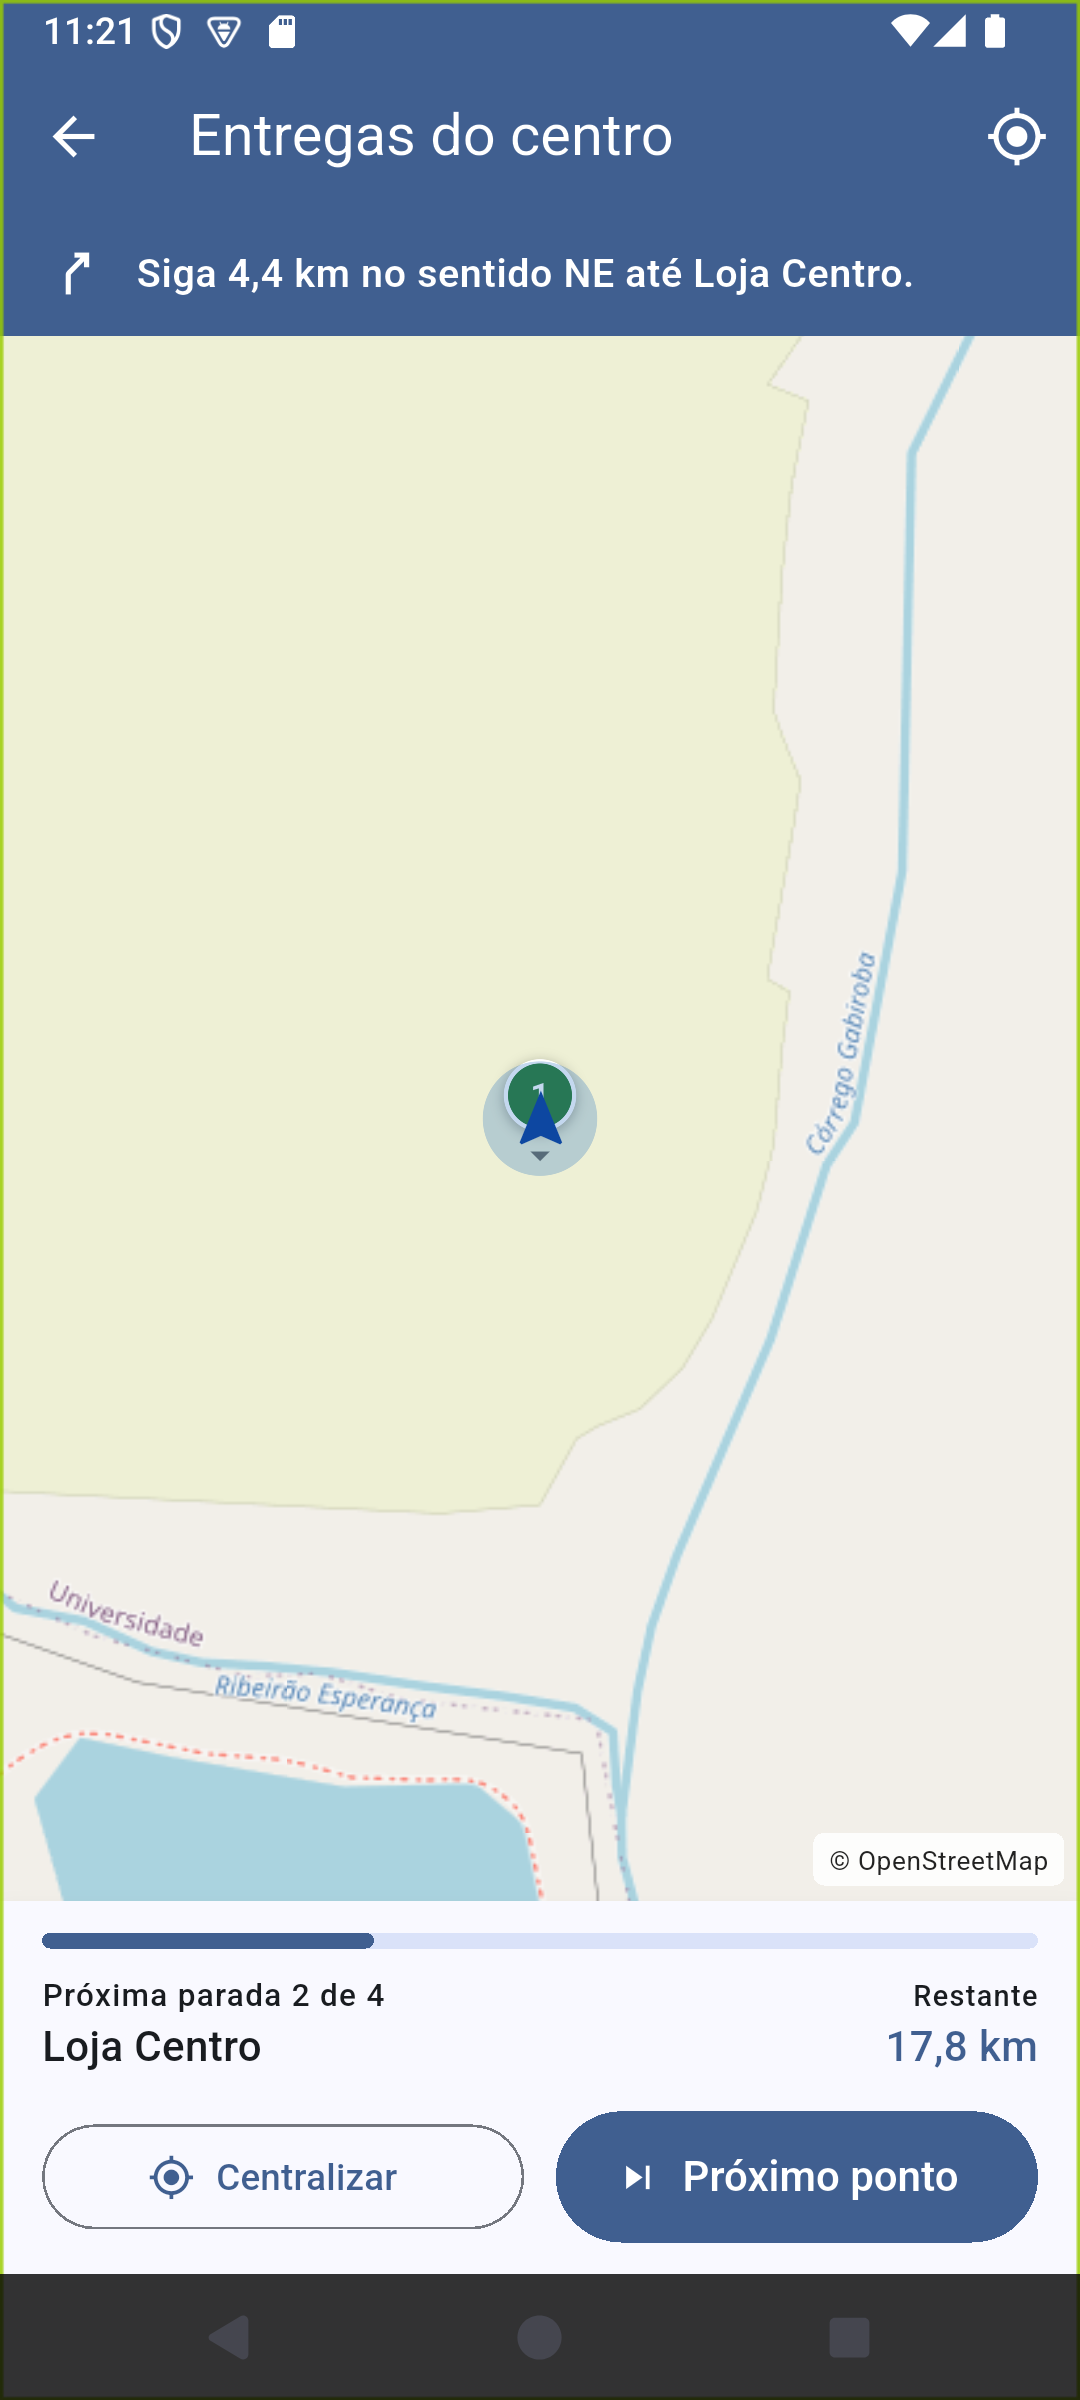
\includegraphics[width=0.5\linewidth]{imagens/tela-navegacao.png}
    \vspace{2pt}
    \footnotesize Fonte: captura do aplicativo em execução (2026)
\end{figure}

\section{Métricas do código-fonte}

A Tabela \ref{tab:metricas-codigo} apresenta o tamanho da versão consolidada, por camada. Os números incluem as linhas de comentários e de documentação das classes, que foram mantidas como parte do artefato entregue.

\begin{table}[!ht]
    \centering
    \caption{Tamanho do código-fonte por camada}
    \label{tab:metricas-codigo}
    \begin{tabular}{p{15cm}rr}
        \hline
        \textbf{Camada} & \textbf{Arquivos} & \textbf{Linhas} \\
        \hline
        Apresentação (telas) & 11 & 2.729 \\
        Serviços & 6 & 1.271 \\
        Persistência (objetos de acesso e banco) & 8 & 950 \\
        Componentes visuais reutilizáveis & 4 & 610 \\
        Infraestrutura (tema, exceções, utilitários e montagem) & 4 & 359 \\
        Modelo de domínio & 3 & 351 \\
        Ponto de entrada e portão de sessão & 2 & 126 \\
        \hline
        \textbf{Total do aplicativo} & \textbf{38} & \textbf{6.396} \\
        \hline
        Testes automatizados & 7 & 1.916 \\
        \hline
    \end{tabular}
    \vspace{2pt}
    \footnotesize Fonte: o próprio autor (2026)
\end{table}

\chapter{Considerações finais}\label{cap:consideracoes-finais}

Este capítulo encerra o relatório apresentando a síntese das atividades desenvolvidas durante o estágio, as dificuldades encontradas no percurso, as limitações identificadas no trabalho realizado e as perspectivas de continuidade do projeto.

\section{Síntese das atividades desenvolvidas}

O estágio teve como resultado o desenvolvimento do S.R.I. -- Sistema de Rotas Inteligentes, aplicativo móvel voltado ao planejamento, à execução e à reutilização de rotas de coleta e entrega. O trabalho foi conduzido segundo o processo RUP, o que implicou a produção dos artefatos de visão, de levantamento de requisitos, de especificação de caso de uso, de especificação complementar e de glossário, além dos modelos de casos de uso, de classes, de entidade e relacionamento, de sequência, de estados e de implantação \cite{kruchten2003}.

Do ponto de vista da implementação, a adoção do framework Flutter permitiu manter uma única base de código para as plataformas Android e iOS, enquanto a persistência local em SQLite assegurou o funcionamento das operações de cadastro e de consulta independentemente da disponibilidade da conexão de rede \cite{flutter2024, sqlite2024}. A integração com os serviços do OpenStreetMap viabilizou a geocodificação de endereços e a representação cartográfica dos pontos cadastrados sem a contratação de chaves de acesso comerciais \cite{osm2024}.

O caso de uso de gerenciamento de locais foi priorizado como primeiro escopo de entrega, por constituir pré-requisito para as funcionalidades de geração de rotas e de rotas salvas \cite{sriEspecUC2026}. A opção por essa ordem de implementação permitiu validar, desde o início do desenvolvimento, a integração entre a interface, a camada de persistência e o serviço externo de geocodificação, que é a base tecnológica compartilhada por todas as demais funcionalidades do sistema. A partir dessa base, foram implementados, na sequência, os casos de uso de geração de rotas, de gerenciamento de rotas salvas e de gerenciamento de usuário, além da navegação assistida, de modo que a versão consolidada contempla a totalidade dos casos de uso previstos no documento de especificação.

\section{Resultados alcançados}

A versão consolidada do S.R.I. contempla os quatro casos de uso previstos na especificação e a funcionalidade de navegação assistida. O gerenciamento de locais permite criar, consultar, atualizar e excluir pontos de interesse, com conversão automática do endereço em coordenadas. A geração de rotas permite compor trajetos nas modalidades ponto a ponto e em circuito, com ordenação automática das paradas, apresentação do traçado sobre o mapa e indicação da distância total e da duração estimada. O gerenciamento de rotas salvas permite gravar, reabrir, alterar e excluir os trajetos calculados. O gerenciamento de usuário impõe a autenticação prévia exigida pelos requisitos e responde pela criação da conta, pela manutenção dos dados cadastrais, pela troca de senha e pela exclusão da conta.

A verificação automatizada produziu resultados objetivos. A análise estática do código-fonte, executada com as regras de estilo configuradas no projeto, não registrou nenhum erro nem aviso. A suíte de testes automatizados, composta por noventa e cinco testes, foi executada integralmente com aprovação. A compilação completa do aplicativo foi concluída com sucesso para o alvo web, confirmando que o conjunto do código-fonte compila de ponta a ponta. O código do aplicativo totaliza 6.047 linhas distribuídas em 37 arquivos, acrescidas de 1.652 linhas de testes.

Quanto à qualidade do algoritmo de ordenação das paradas, o teste comparativo com a solução ótima obtida por força bruta, em uma instância de cinco pontos, confirmou que a solução heurística não excede o ótimo em mais de quinze por cento, além de nunca ser pior que a ordem produzida isoladamente pela heurística construtiva.

Duas métricas de aceitação declaradas nos requisitos permanecem pendentes de medição em campo. A primeira é o tempo de resposta das operações de geocodificação e de cálculo de trajeto, que o projeto limita em trinta segundos: o limite de tempo das requisições foi configurado em vinte segundos justamente para assegurar esse teto, mas a medição efetiva depende da latência real dos serviços externos em condições de uso. A segunda é o patamar de assertividade de setenta por cento nas rotas geradas, que depende da validação das rotas junto ao usuário do sistema e não pode ser aferido apenas por testes automatizados \cite{sriEspecComp2025, sriPedido2025}.

\section{Dificuldades encontradas}

A primeira dificuldade decorreu da assimetria entre o esforço de documentação e o tempo disponível para implementação. A adoção do RUP, com a produção de artefatos formais em cada disciplina, mostrou-se valiosa para o entendimento do domínio, mas exigiu um volume de trabalho de escrita que competiu diretamente com as horas destinadas ao desenvolvimento. O aprendizado obtido foi o de dimensionar o nível de detalhe da documentação conforme o risco do requisito, aprofundando os artefatos das funcionalidades centrais e mantendo mais enxutos aqueles de menor incerteza \cite{kruchten2003}.

A segunda dificuldade esteve relacionada à integração com os serviços externos de geocodificação e de roteamento. Tais serviços impõem limites de uso e apresentam variação no tempo de resposta, o que exigiu o tratamento explícito de situações de falha e de espera prolongada na interface, com a exibição de indicadores de carregamento e de mensagens de erro compreensíveis ao usuário \cite{nominatim2024, osrm2024}.

A terceira dificuldade foi de natureza algorítmica. A definição da estratégia de ordenação das paradas exigiu o estudo das heurísticas de roteirização e a avaliação de seu custo computacional no dispositivo, uma vez que a obtenção da solução ótima é inviável para instâncias de tamanho realista \cite{cunha2000}. A solução adotada combinou uma heurística construtiva com um método de refinamento, o que demandou a construção de testes específicos para verificar a corretude da ordenação produzida \cite{croes1958}.

\section{Limitações}

A principal limitação identificada é a dependência de conectividade para as funcionalidades que exigem geocodificação de endereços e cálculo de rota sobre a malha viária. O cadastro e a consulta de locais permanecem operacionais sem conexão, mas a conversão de um novo endereço em coordenadas e a obtenção de um trajeto por vias exigem acesso à rede, conforme estabelecido nas premissas e dependências do produto \cite{sriVisao2025}.

Uma segunda limitação decorre do escopo funcional da navegação assistida. A funcionalidade mantém o motorista informado sobre a próxima parada e o quanto falta para alcançá-la, mas não recalcula o trajeto quando o veículo se desvia da malha viária prevista nem emite comandos de voz, recursos presentes em soluções comerciais de navegação. A verificação funcional em aparelho físico, com variação real da precisão do sinal de GPS e instabilidade da rede móvel, também permanece pendente, tendo a validação automatizada se limitado aos cálculos de navegação e às regras de negócio \cite{sriEspecComp2025}.

Registra-se ainda que os testes foram executados em ambiente de emulador, o que, embora permita verificar o comportamento das telas, das permissões de localização e da persistência, não reproduz integralmente as condições de uso em campo, como a variação da precisão do sinal de GPS e a instabilidade da rede móvel.

\section{Trabalhos futuros}

Como continuidade do projeto, estão previstas a medição das métricas de aceitação ainda pendentes, com o registro dos tempos de resposta das operações de geocodificação e de cálculo de trajeto e com a validação das rotas geradas junto ao usuário do sistema, de modo a consolidar a avaliação de assertividade \cite{sriPedido2025}; a realização de testes em dispositivo físico, em condições reais de operação, para aferir o comportamento da geolocalização, o consumo de bateria e o desempenho com o banco de dados já populado; e a ampliação da suíte de testes automatizados, com a cobertura dos fluxos de interface hoje verificados apenas manualmente.

No curto prazo, uma evolução de baixo custo é o emprego da geometria já gravada no cálculo da distância restante durante a navegação, em lugar da distância em linha reta hoje utilizada, o que aproximaria a estimativa apresentada ao motorista da distância efetivamente percorrida sobre as vias.

No médio prazo, o documento de Visão prevê a inclusão de recursos de visualização do tráfego em tempo real, o compartilhamento de rotas por link e a integração com aplicativos de entrega e com sistemas de gestão logística \cite{sriVisao2025}. Outra evolução considerada é a substituição da heurística de ordenação por métodos de busca local mais elaborados, com o objetivo de reduzir a distância total dos circuitos gerados.

\section{Considerações finais}

O desenvolvimento do S.R.I. proporcionou a aplicação integrada dos conteúdos estudados ao longo do curso, articulando engenharia de software, modelagem de sistemas, banco de dados, algoritmos e programação para dispositivos móveis em torno de um problema real, apresentado por um usuário real e com critérios de aceitação declarados. A experiência evidenciou que a qualidade do resultado depende menos da escolha da tecnologia do que da clareza dos requisitos e da consistência entre o processo de negócio documentado e as funcionalidades efetivamente implementadas.

Do ponto de vista formativo, o estágio consolidou a compreensão de que o desenvolvimento de software é uma atividade de engenharia, na qual decisões de escopo, de modelagem e de validação precisam ser tomadas de forma explícita e registrada. A documentação produzida ao longo do período, além de atender às exigências acadêmicas do estágio obrigatório, constitui o principal instrumento de continuidade do projeto, uma vez que permite que o trabalho seja retomado sem a necessidade de reconstruir o entendimento do domínio \cite{sommerville2019}.


\cleardoublepage

\postextual

\bibliography{bibliografia}{}

\end{document}
